\documentclass{article}

\usepackage{hcmut-report}
\usepackage{codespace}

% Sub-preambles
% https://github.com/MartinScharrer/standalone
% Encodings
\usepackage{amsmath,amssymb,gensymb,textcomp}

% Better tables
% Wide tables go to https://tex.stackexchange.com/q/332902
\usepackage{array,multicol,multirow,siunitx,tabularx}

% Better enum
\usepackage{enumitem}

% Graphics
\usepackage{caption,float}

% Allow setting >max< width of figure
% Remove if unneeded
\usepackage[export]{adjustbox} % 'export' allows adjustbox keys in \includegraphics
\usepackage{mwe}

\documentclass{article}
\usepackage{listings}
\usepackage{xcolor}

\definecolor{codegreen}{rgb}{0,0.6,0}
\definecolor{codegray}{rgb}{0.5,0.5,0.5}
\definecolor{codepurple}{rgb}{0.58,0,0.82}
\definecolor{backcolour}{rgb}{0.95,0.95,0.92}

\lstdefinestyle{mystyle}{
    backgroundcolor=\color{backcolour},   
    commentstyle=\color{codegreen},
    keywordstyle=\color{magenta},
    numberstyle=\tiny\color{codegray},
    stringstyle=\color{codepurple},
    basicstyle=\ttfamily\footnotesize,
    breakatwhitespace=false,         
    breaklines=true,                 
    captionpos=b,                    
    keepspaces=true,                 
    numbers=left,                    
    numbersep=5pt,                  
    showspaces=false,                
    showstringspaces=false,
    showtabs=false,                  
    tabsize=2
}

\lstset{style=mystyle}
% Custom commands
% Remove if unneeded
\newcommand*\mean[1]{\bar{#1}}
\ocoursename{CO3071 - DISTRIBUTED SYSTEMS}
\oreporttype{CC01 - GROUP 05 - ASSIGNMENT REPORT}
\title{\huge{Deploy a Three-Tier Web Application}}
%\oreporttype{In-depth analysis and evaluation of Students' Performance among various factors with Multi-factor ANOVA Test and Multiple Linear Regression Models using R}
%In-depth analysis and evaluation of Students' Performance among various factors with Multi-factor ANOVA Test and Multiple Linear Regression Models using R
\oadvisor{Nguyen Khanh Nam - 2153599}
\oinstructor{\textbf{PROF. Thoai Nam}}

\reportlayout%

\begin{document}

\coverpage%

\tableofcontents

\newpage

\section{Introduction}
In the ever-evolving landscape of information technology, the design and deployment of distributed systems play a pivotal role in meeting the demands of scalable, efficient, and resilient applications. The Distributed Systems course provides a comprehensive exploration of the principles, challenges, and practical implementations of distributed computing. As part of this course, this report delves into the hands-on experience of deploying a 3-tier architecture, a fundamental and widely adopted design pattern, utilizing the robust infrastructure of Amazon Web Services (AWS).\par
\begin{figure}[h]
    \centering
    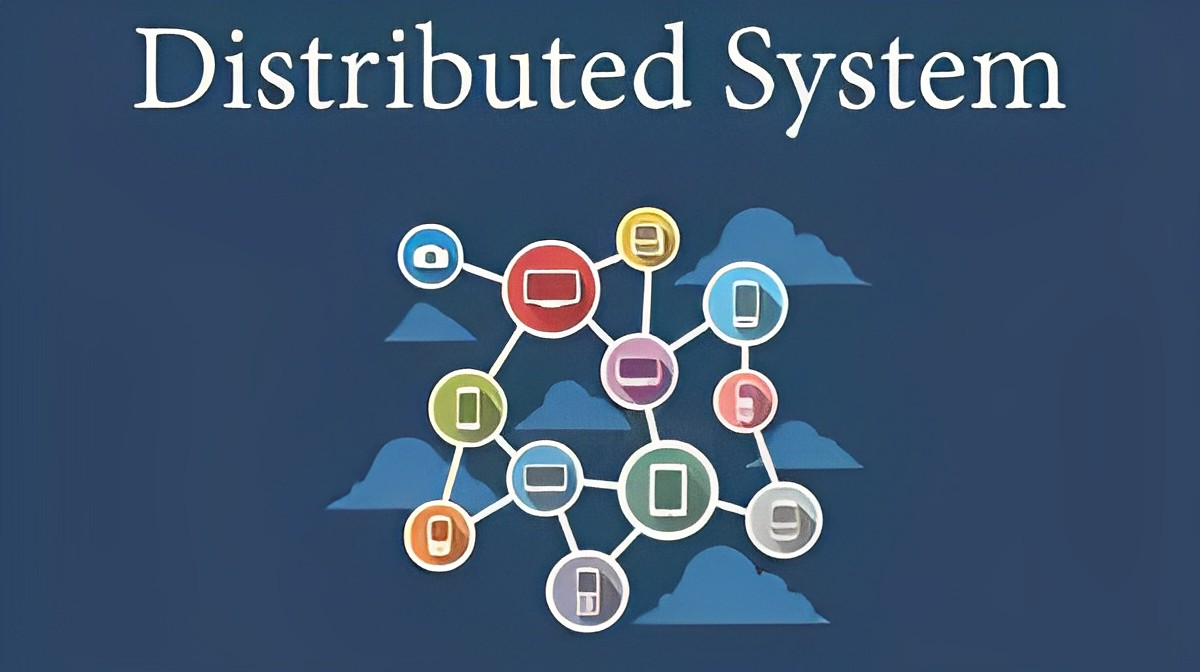
\includegraphics[width=13cm]{Pictures/Introduction/DSs intro.jpg}
    \caption{Distributed Systems.}
    \label{fig:enter-label}
\end{figure}
The 3-tier architecture, consisting of presentation, application, and data layers, stands as a timeless model for building robust and scalable web applications. Its modular structure not only facilitates ease of development but also enables efficient scaling and maintenance. By delving into the deployment of this architecture within the AWS environment, students gain practical insights into how cloud services enhance the traditional 3-tier model, paving the way for the creation of dynamic, responsive, and globally accessible applications.\par
\begin{figure}[h]
    \centering
    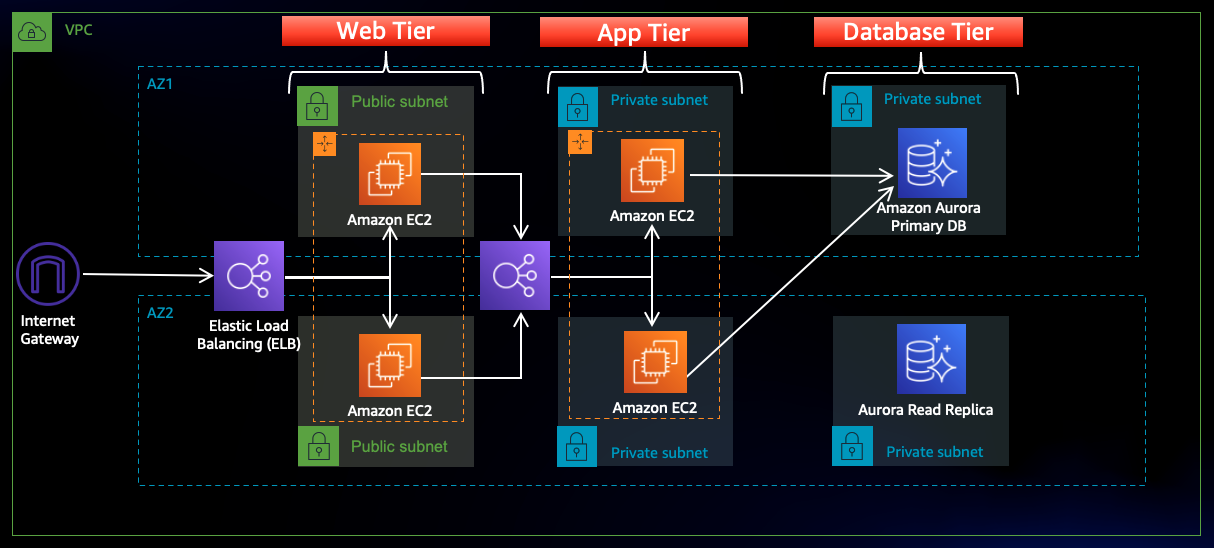
\includegraphics[width = 13cm]{Pictures/Introduction/3TierArch.png}
    \caption{Three-Tier Architect using AWS.}
    \label{fig:enter-label}
\end{figure}
\newpage

\section{Theoretical Basis}
\subsection{Amazon Web Service}
Amazon Web Services (AWS) is a comprehensive and widely adopted cloud computing platform provided by Amazon.com. Launched in 2006, AWS has rapidly grown into a global leader in the cloud services industry, offering a vast array of computing resources, storage options, and scalable solutions for businesses, developers, and organizations.\par
\vspace{10pt}
\textbf{Benefits of AWS:}\par
\begin{itemize}
    \item Scalability: Easily scale resources up or down based on demand.
    \item Cost-Efficiency: Pay only for the resources you consume, reducing upfront capital expenses.
    \item Global Reach: AWS operates in multiple regions globally, providing low-latency access to resources.
    \item Security and Compliance: Robust security measures and compliance certifications ensure the protection of data and adherence to industry standards.
    \item Innovation: Continuous introduction of new services and features to stay at the forefront of technological advancements.
\end{itemize}

\begin{figure}[h]
    \centering
    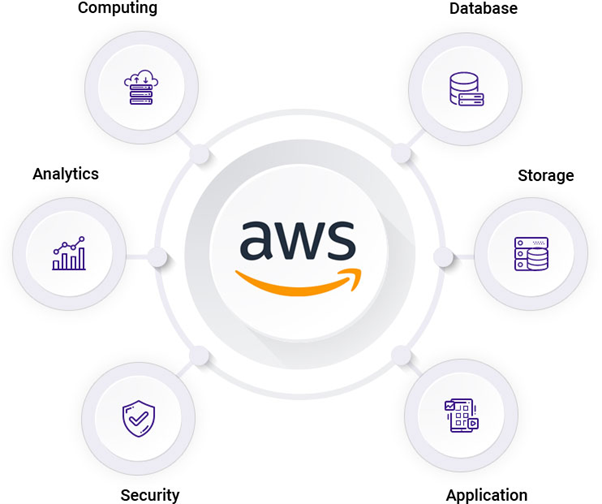
\includegraphics[width = 10cm]{Pictures/Theory/AWS.png}
    \caption{Amazon Web Service.}
    \label{fig:enter-label}
\end{figure}

\subsection{Regions and Availability Zones}
\textbf{Regions}\par
\vspace{10pt}
AWS has Regions all around the world. Names can be us-east-1, eu-west-3...\par
A region is a cluster of data centers. Most AWS services are region-scope.\par
\newpage
\textbf{Availability Zones}\par
\vspace{10pt}
Each region has many availability zones (usually 3, min is 3, max is 6). Example:\par
\begin{itemize}
    \item ap-southeast-2a
    \item ap-southeast-2b
    \item ap-southeast-2c
\end{itemize}
  \par
Each availability zone (AZ) is one or more discrete data centers with redundant power, networking, and connectivity.\par
They’re separate from each other, so that they’re isolated from disasters.\par
They’re connected with high bandwidth, ultra-low latency networking.\par
\begin{figure}[h]
    \centering
    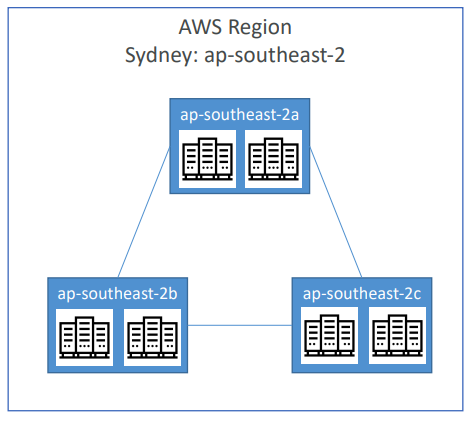
\includegraphics[width = 10cm]{Pictures/Theory/Regions and AZs.png}
    \caption{Regions and Availability Zones.}
    \label{fig:enter-label}
\end{figure}

\subsection{Identity and Access Management (IAM)}
\textbf{IAM: Users \& Groups}\par
\begin{itemize}
    \item IAM = Identity and Access Management, Global service.
    \item Root account created by default, shouldn’t be used or shared.
    \item Users are people within your organization, and can be grouped.
    \item Groups only contain users, not other groups.
    \item Users don’t have to belong to a group, and user can belong to multiple groups.
\end{itemize}
\begin{figure}[h]
    \centering
    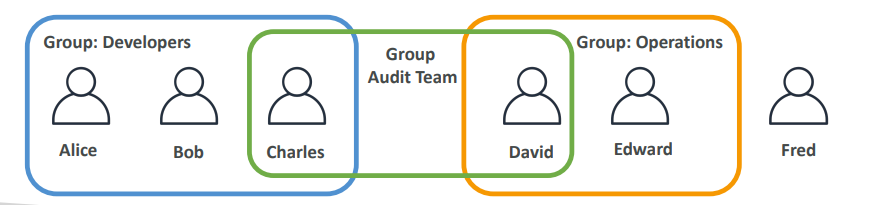
\includegraphics[width = 13cm]{Pictures/Theory/IAM_Define.png}
    \caption{How IAM work.}
    \label{fig:enter-label}
\end{figure}

\textbf{IAM: Permissions}\par
\begin{itemize}
    \item Users or Groups can be assigned JSON documents called policies.
    \item These policies define the permissions of the users.
    \item In AWS you apply the least privilege principle: don’t give more permissions than a user needs.
\end{itemize}
\begin{figure}[h]
    \centering
    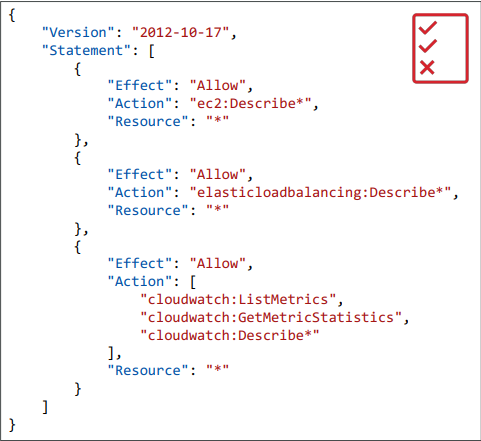
\includegraphics[width = 7cm]{Pictures/Theory/IAM_JSON.png}
    \caption{Example of a JSON file.}
    \label{fig:enter-label}
\end{figure}

\textbf{IAM: Roles for Services}\par
\begin{itemize}
    \item Some AWS services will need to perform actions on your behalf.
    \item To do so, we will assign permissions to AWS services with IAM Roles.
    \item Common roles: \textbf{EC2 Instance Roles}, Lambda Function Roles, Roles for CloudFormation 
\end{itemize}

\begin{figure}[h]
    \centering
    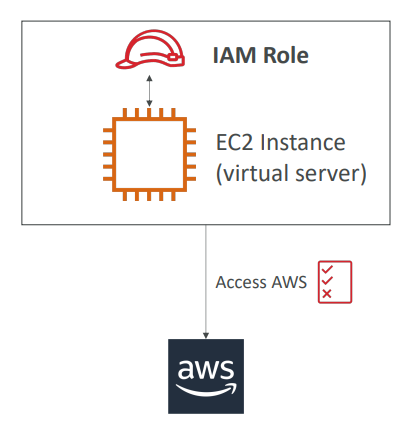
\includegraphics[width = 5cm]{Pictures/Theory/IAM_Roles.png}
    \caption{Given roles to an EC2 Instance.}
    \label{fig:enter-label}
\end{figure}
\newpage

\subsection{Amazon S3}
Amazon S3, or Amazon Simple Storage Service, is a scalable and highly durable object storage service offered by Amazon Web Services (AWS). It is designed to store and retrieve any amount of data from anywhere on the web and is commonly used for a variety of use cases, ranging from simple storage to complex data analytics. It’s advertised as ”infinitely scaling” storage.\par 
Many websites use Amazon S3 as a backbone. Many AWS services use Amazon S3 as an integration as well.\par
\textbf{Key concepts}\par
\begin{itemize}
    \item Buckets: The fundamental container for data storage in S3. Each bucket must have a globally unique name and can contain an unlimited number of objects.
    \item Objects: Objects are the data entities stored in S3. They consist of data, a key (unique within a bucket), and metadata.
\end{itemize}
\begin{figure}[h]
    \centering
    
\includegraphics[width = 10cm]{Pictures/Theory/Amazon S3.png}
    \caption{Amazon S3.}
    \label{fig:enter-label}
\end{figure}

\textbf{Use cases: } Backup and storage, disaster recovery, archive, hybrid cloud storage, application hosting, media hosting, data lakes \& big data analytics, software delivery, static website,\par

Amazon S3 allows people to store objects (files) in “buckets” (directories). Buckets must have a globally unique name (across all regions all accounts). Buckets are defined at the region level.\par
S3 looks like a global service but buckets are created in a region.\par
\begin{figure}[h]
    \centering
    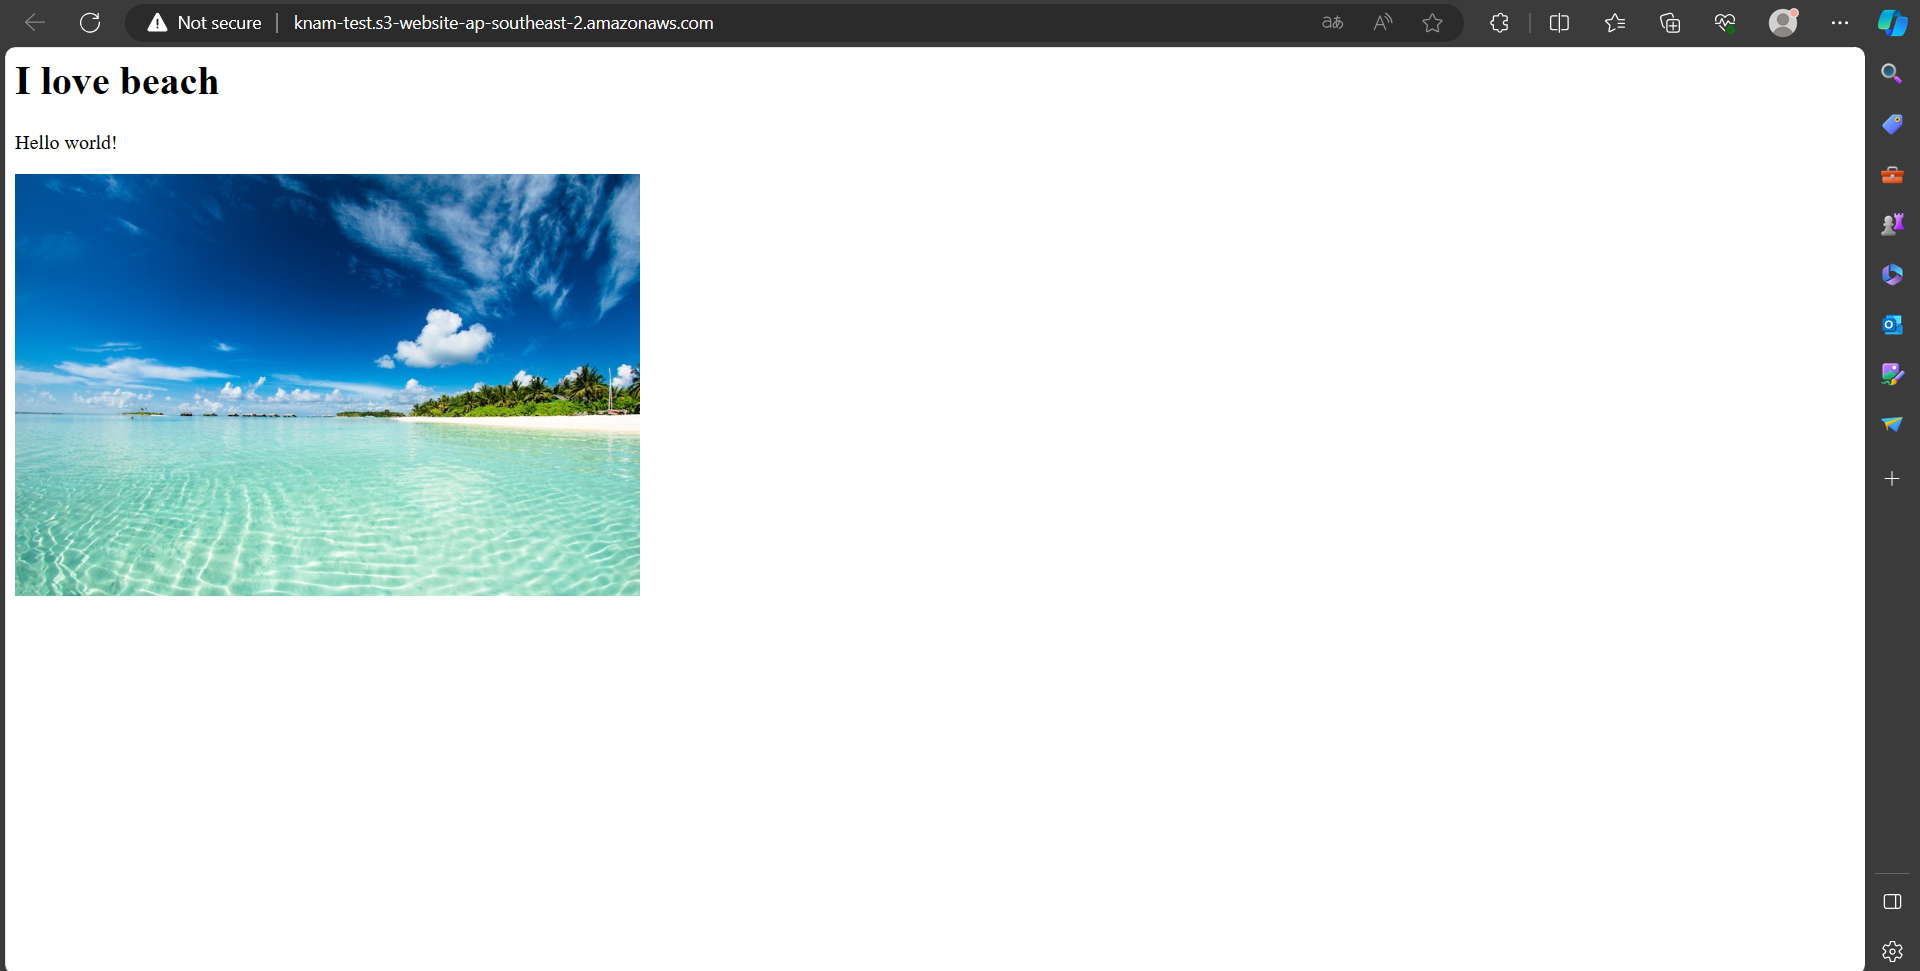
\includegraphics[width=13cm]{Pictures/Theory/Static Web S3.png}
    \caption{Hosting a static website using S3.}
    \label{fig:enter-label}
\end{figure}
\newpage

\subsection{Amazon RDS}
Amazon RDS (Relational Database Service) is a fully managed database service provided by AWS. It simplifies the process of setting up, operating, and scaling relational databases in the cloud. RDS supports various database engines such as MySQL, PostgreSQL, Oracle, SQL Server, and MariaDB.\par
With features like automated backups, patch management, and automatic failover, RDS allows users to focus on application development while AWS handles routine database administration tasks. It provides a scalable and highly available solution for deploying and managing relational databases in the cloud.\par
\begin{figure}[h]
    \centering
    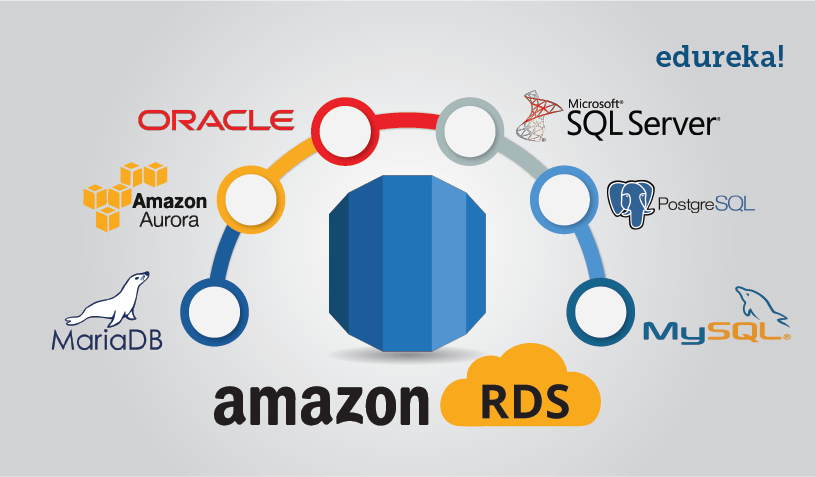
\includegraphics[width=12cm]{Pictures/Theory/AWS-RDS.png}
    \caption{Amazon RDS.}
    \label{fig:enter-label}
\end{figure}
\textbf{Replication using Amazon RDS: }RDS provides robust database replication options, allowing users to create replicas for read scalability, disaster recovery, and high availability. With features like Multi-AZ deployments and Read Replicas, RDS simplifies and automates the process of replicating databases, enhancing performance and resilience.\par
\begin{figure}[h]
    \centering
    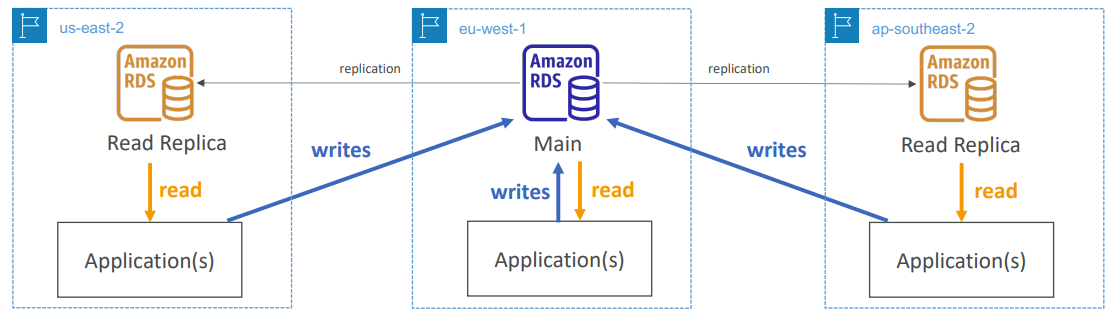
\includegraphics[width=13cm]{Pictures/Theory/RDS Replicate.png}
    \caption{Read replicas RDS deployment.}
    \label{fig:enter-label}
\end{figure}
\newpage

\subsection{Elastic Compute Cloud}
Amazon Elastic Compute Cloud (EC2) is a web service provided by Amazon Web Services (AWS) that enables users to rent virtual servers, known as instances, on-demand. EC2 provides scalable compute capacity in the cloud, allowing users to quickly deploy and manage applications, handle varying workloads, and scale resources as needed. It's a foundational service in AWS, offering a wide range of instance types optimized for different use cases, along with features like auto-scaling, security groups, and Elastic Load Balancing for enhanced flexibility and performance.\par
\begin{figure}[h]
    \centering
    
\includegraphics[width=7cm]{Pictures/Theory/amazon_ec2.png}
    \caption{Amazon Elastic Cloud Compute.}
    \label{fig:enter-label}
\end{figure}
\subsubsection{EC2 Instances}
An EC2 instance in AWS, part of Amazon Elastic Compute Cloud (EC2), is a virtual server in the cloud that users can rent on-demand. EC2 instances provide scalable compute capacity and allow users to run applications, host websites, and perform various computing tasks in a flexible and cost-effective manner. Users can choose from a variety of instance types optimized for different workloads, and they have full control over the configuration, security, and scaling of their instances.\par
\begin{figure}[h]
    \centering
    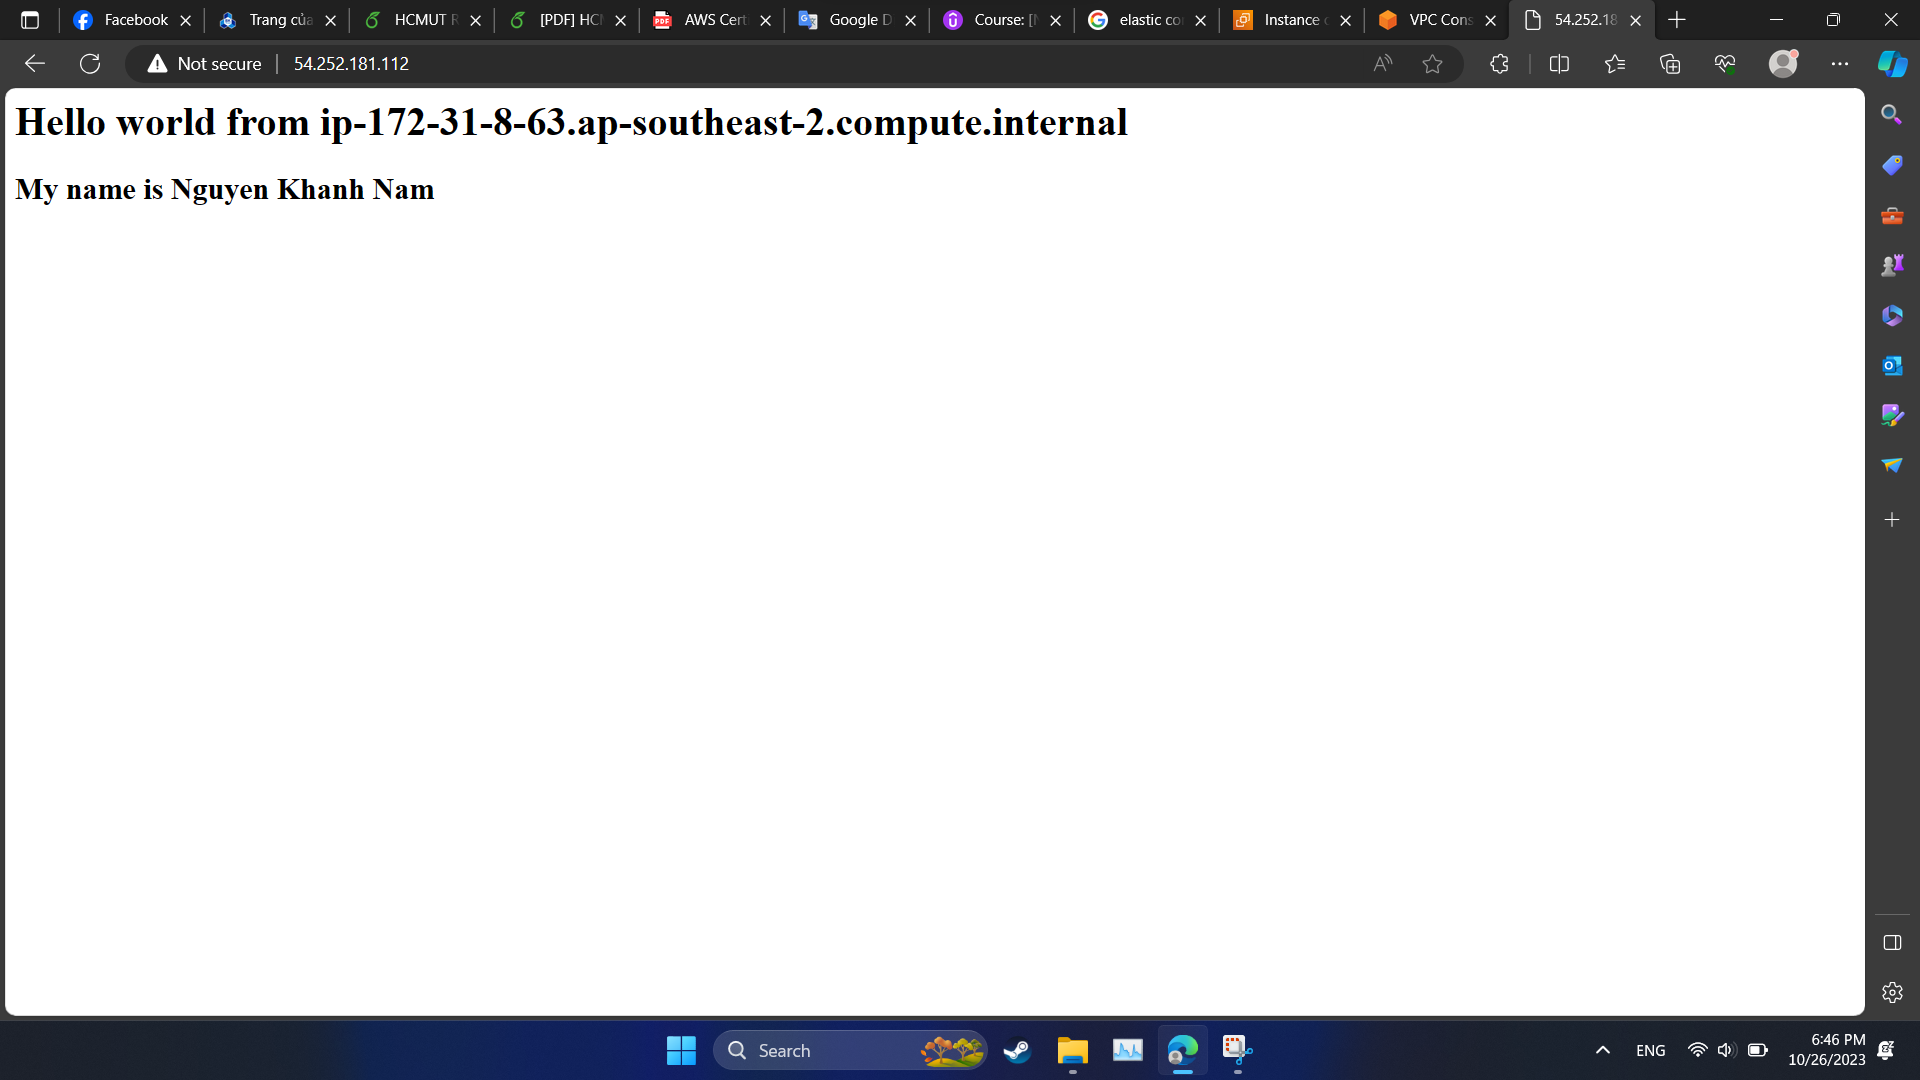
\includegraphics[width=13cm]{Pictures/Theory/EC2 web.png}
    \caption{Hosting a web server using t2.micro instance.}
    \label{fig:enter-label}
\end{figure}
\textbf{EC2 Instances Purchasing Options: }On-Demand Instances, Reserved (1 \& 3 years), Reserved Instances, Convertible Reserved Instances, Savings Plans (1 \& 3 years), Spot Instances, Dedicated Hosts, Dedicated Instances, Capacity Reservations.\par
\newpage
\textbf{EC2 Instance Types}\par
\vspace{10pt}
EC2 instance types in AWS refer to various virtual server configurations optimized for different use cases. They vary in terms of compute, memory, storage, and networking capacities. Users can choose instance types that best match their specific application requirements, allowing for flexibility and cost optimization.\par
Common families include General Purpose (e.g., t3), Compute Optimized (e.g., c5), Memory Optimized (e.g., r5), and Storage Optimized (e.g., i3). Each family caters to specific performance needs, providing a diverse range of options for deploying applications in the cloud.\par
\begin{figure}[h]
    \centering
    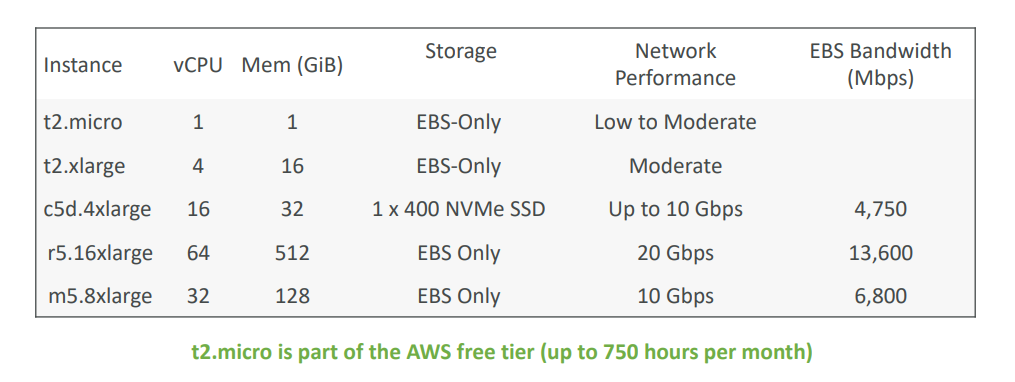
\includegraphics[width=13cm]{Pictures/Theory/EC2 instance types.png}
    \caption{Example of Instance Types.}
    \label{fig:enter-label}
\end{figure}
\subsubsection{Elastic Load Balancing}
\textbf{Scalability: }  Scalability means that an application / system can handle greater loads by adapting. There are two kinds of scalability:
\begin{itemize}
    \item Vertical Scalability
    \item Horizontal Scalability (elasticity)
\end{itemize}
\begin{figure}[H]
  \centering
  \begin{minipage}[b]{0.4\textwidth}
    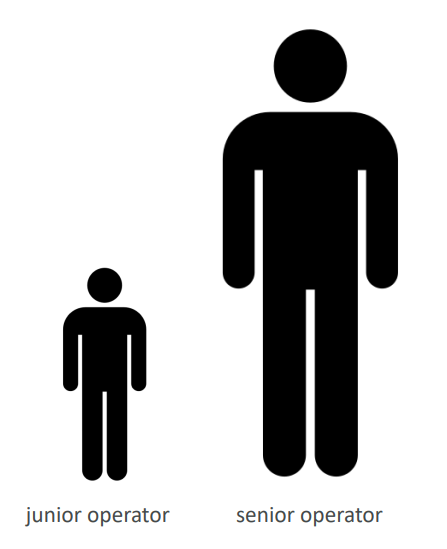
\includegraphics[width=5cm]{Pictures/Theory/Vertical scale.png}
    \caption{Vertical Scale.}
  \end{minipage}
  \hfill
  \begin{minipage}[b]{0.4\textwidth}
    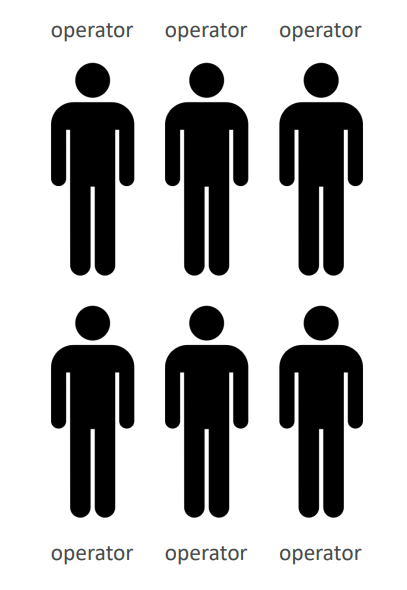
\includegraphics[width=5cm]{Pictures/Theory/Horizontal Scale.png}
    \caption{Horizontal Scale.}
  \end{minipage}
\end{figure}

\textbf{Scalability is linked but different to High Availability: } High Availability usually goes hand in hand with horizontal scaling. High availability means running your application / system in at  least 2 Availability Zones. The goal of high availability is to survive a data center loss (disaster).\par

\begin{figure}[h]
    \centering
    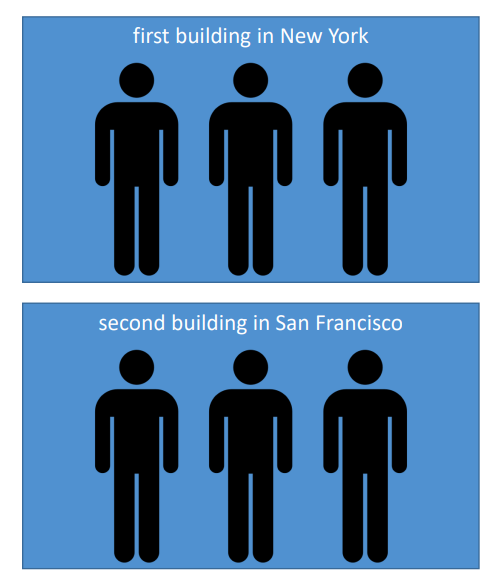
\includegraphics[width=7cm]{Pictures/Theory/High availability.png}
    \caption{High availability.}
    \label{fig:enter-label}
\end{figure}


\textbf{Elastic Load Balancing (ELB) }in AWS is a fully managed service that automatically distributes incoming application traffic across multiple EC2 instances. It enhances fault tolerance, increases availability, and ensures even distribution of workloads. ELB supports various load balancing algorithms and seamlessly scales to handle varying levels of traffic, providing a reliable and efficient solution for managing application traffic in the cloud.\par
\begin{figure}[h]
    \centering
    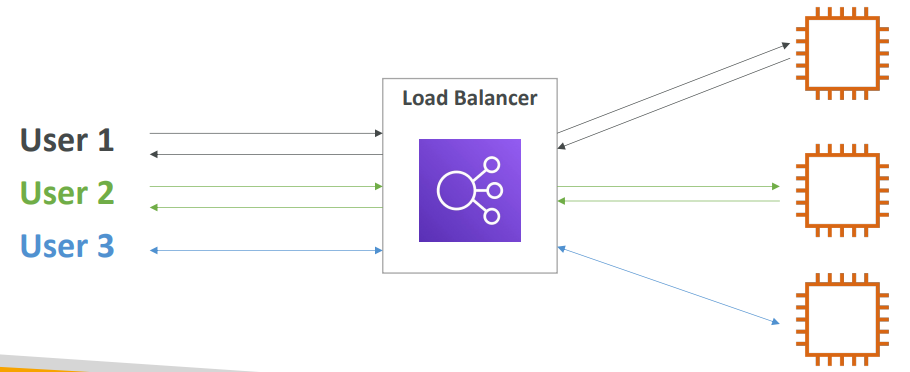
\includegraphics[width=10cm]{Pictures/Theory/ELB.png}
    \caption{Elastic Load Balancing.}
    \label{fig:enter-label}
\end{figure}

\subsubsection{Auto Scaling Group}
Auto Scaling Group (ASG) in AWS is a service that automatically adjusts the number of EC2 instances in a group based on defined policies or conditions. It helps maintain application availability and ensures optimal performance by automatically scaling instances in and out to meet varying workloads.\par
ASG allows users to define minimum and maximum instance counts, set up scaling policies, and seamlessly integrate with other AWS services. This dynamic scaling capability enhances reliability and cost efficiency, as resources can automatically adapt to changes in demand.\par
\begin{figure}[h]
    \centering
    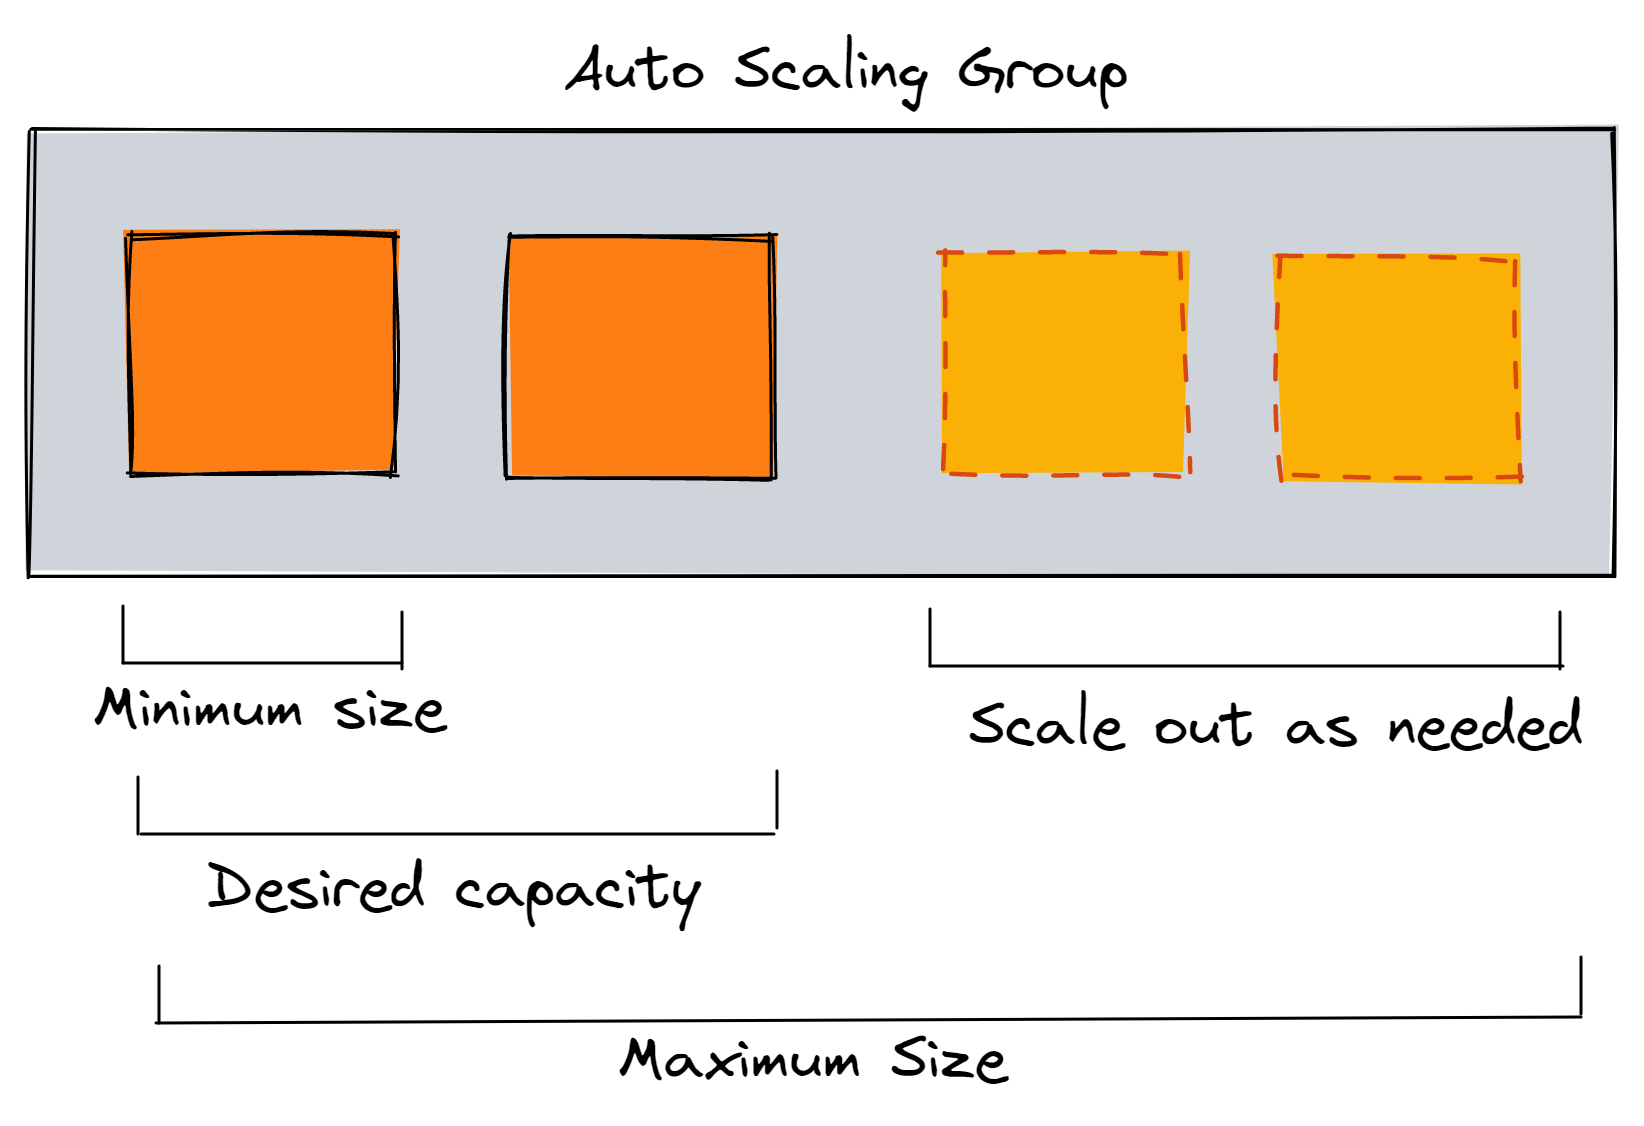
\includegraphics[width=13cm]{Pictures/Theory/AWS ASG.png}
    \caption{How ASG work.}
    \label{fig:enter-label}
\end{figure}
\newpage

\subsection{Network and Security}
AWS provides a robust set of networking services, allowing users to create, configure, and manage virtual networks. Amazon VPC (Virtual Private Cloud) enables users to launch resources in a logically isolated section of the AWS Cloud.\par
Security is a top priority in AWS, with a shared responsibility model where AWS manages the security of the cloud infrastructure, and customers are responsible for securing their data within it.\par
\begin{figure}[!htp]
    \centering
    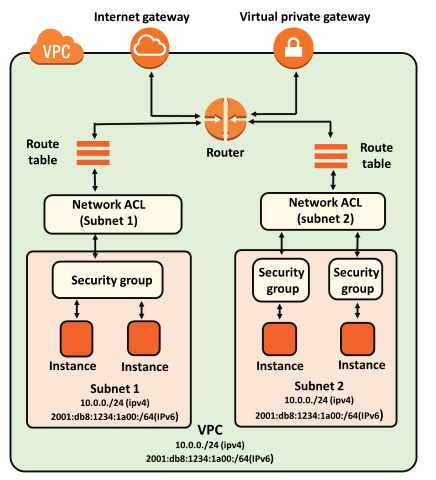
\includegraphics[width=8cm]{Pictures/Theory/Network and Security.png}
    \caption{Network and Security in AWS.}
    \label{fig:enter-label}
\end{figure}
\newpage
\subsubsection{Virtual Private Cloud (VPC)}
Amazon Virtual Private Cloud (VPC) is a service that allows you to create a logically isolated section of the AWS Cloud where you can launch AWS resources in a virtual network that you define. With VPC, you have complete control over your network configuration, including IP address ranges, subnets, routing tables, and security settings. It provides a secure and scalable foundation for deploying applications, offering features such as private and public subnets, network access control lists (ACLs), and the ability to connect your VPC to your on-premises network or other VPCs. VPC enables you to build a customized, isolated, and highly flexible network environment in the AWS Cloud.\par

\subsubsection{Subnets}
Subnets are subdivisions of an Amazon VPC's IP address range. They allow you to segment your VPC's address space to organize and secure your resources. Resources within the same subnet can communicate directly, and you can apply different network and security policies to each subnet. Subnets can be public (accessible from the internet) or private (not accessible from the internet).\par

\subsubsection{Route Table}
In AWS, a route table is a networking component that defines the rules for routing traffic within a Virtual Private Cloud (VPC). It contains a set of rules, known as routes, that determine the paths traffic takes. Each subnet in a VPC must be associated with a route table, which controls the traffic leaving and entering the subnet. Route tables play a crucial role in directing network traffic to its destination, including defining routes to internet gateways, virtual private gateways, or other network destinations within the VPC.\par
\subsubsection{Security Groups}
In AWS, a security group acts as a virtual firewall for your instances to control inbound and outbound traffic. It essentially functions as a set of rules that govern how traffic is allowed or denied to and from instances. Security groups are associated with instances and operate at the instance level, providing a flexible and scalable way to manage network access. They enable you to specify rules based on protocols, ports, and source or destination IP addresses, helping ensure a secure and controlled environment for your AWS resources.\par
\newpage

\section{Implementation}
\subsection{Setup}
First of all, we must create our bucket to store the files of our application. Navigating to the S3 in the console to access the Amazon S3, then we will start to create the bucket. Select the bucket's name as \textbf{distributed-systems-assignment} bucket and it will be located in the Sydney region due to the near distance.\par
\begin{figure}[h]
    \centering
    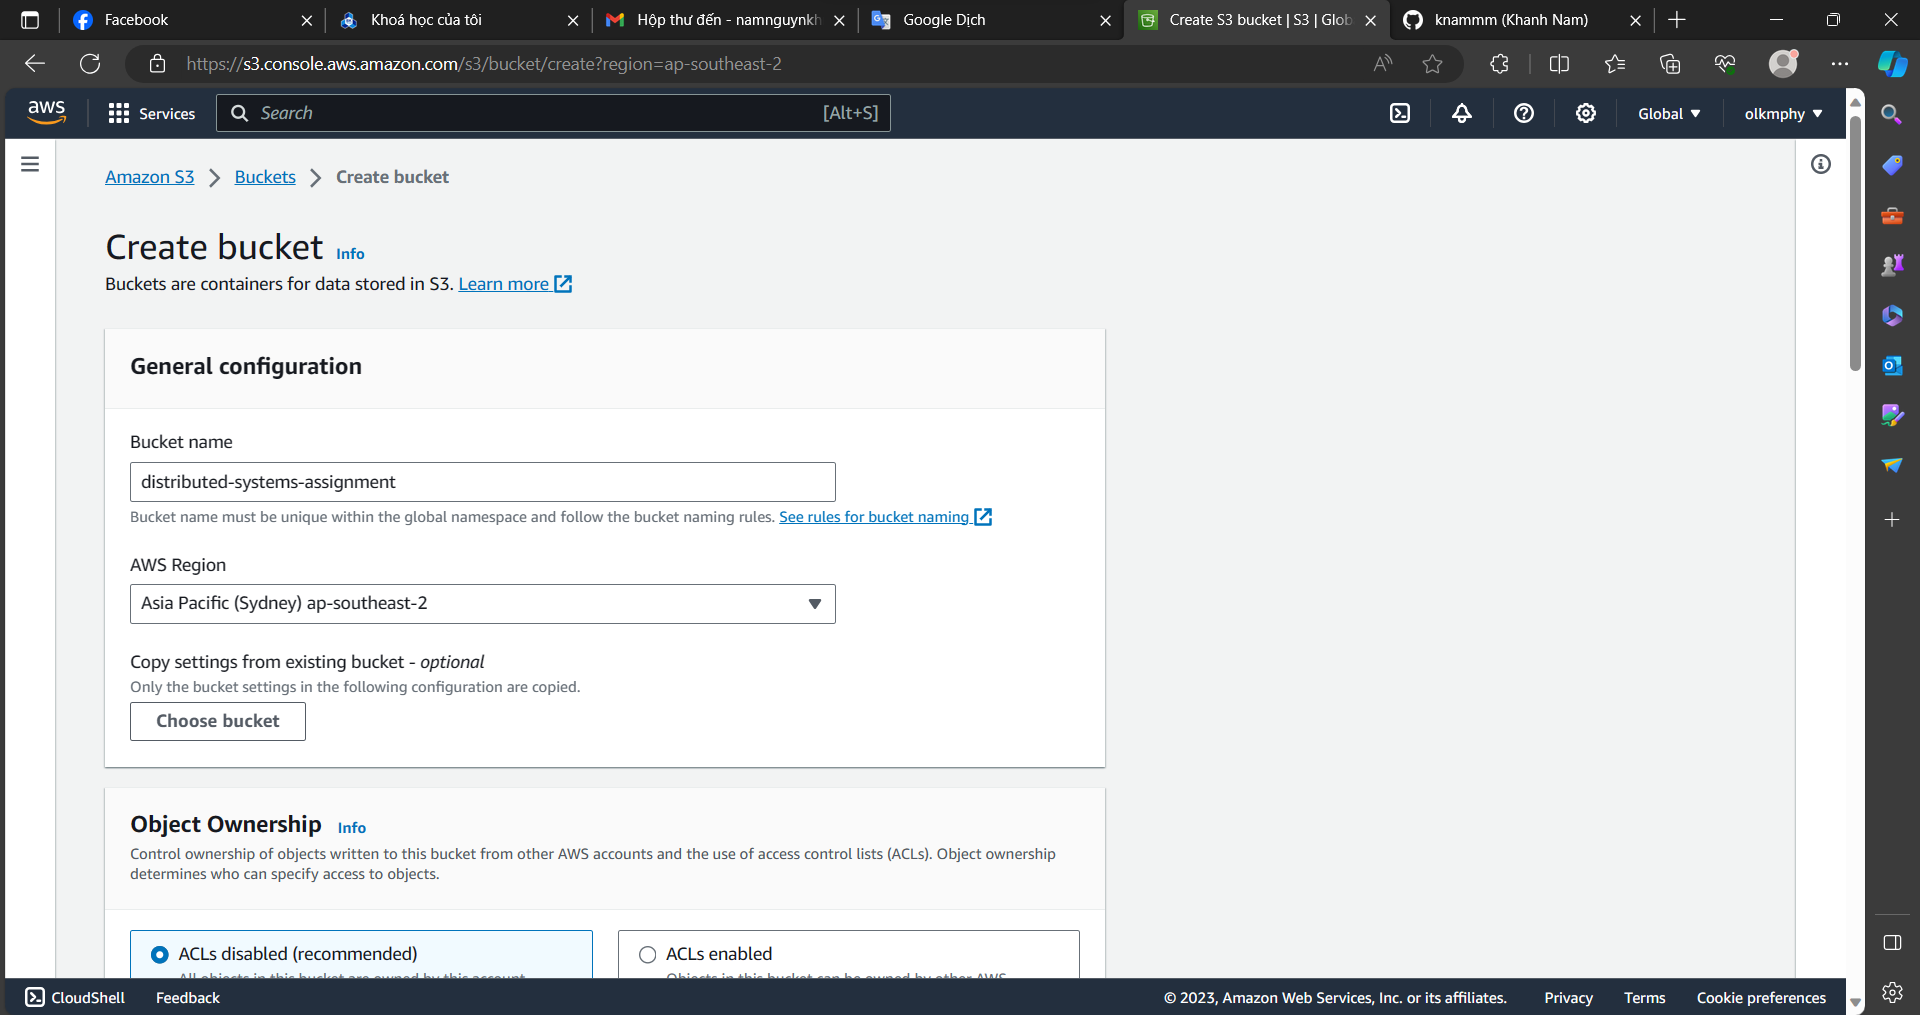
\includegraphics[width=12cm]{Pictures/Set up/S3-create.png}
    \caption{Create S3 bucket.}
    \label{fig:enter-label}
\end{figure}
Next step is to create the IAM role that will be attached to an EC2 instace. I will name it as \textbf{Distributed\_Systems\_Assignment\_IAM\_Roles} and it will contain two specific roles which are:
\begin{itemize}
    \item \textbf{AmazonS3ReadOnlyAccess}
    \item \textbf{AmazonSSMManagedInstanceCore}
\end{itemize}
\vspace{10pt}
The \textit{AmazonS3ReadOnlyAccess} will help our instance to read the bucket's content so that we can download our code from the bucket. The second role which is called \textit{AmazonSSMManagedInstanceCore}. This role uses Systems Manager to help us connect securely to the instance without using the SSH keys through the AWS console.\par
\begin{figure}[h]
    \centering
    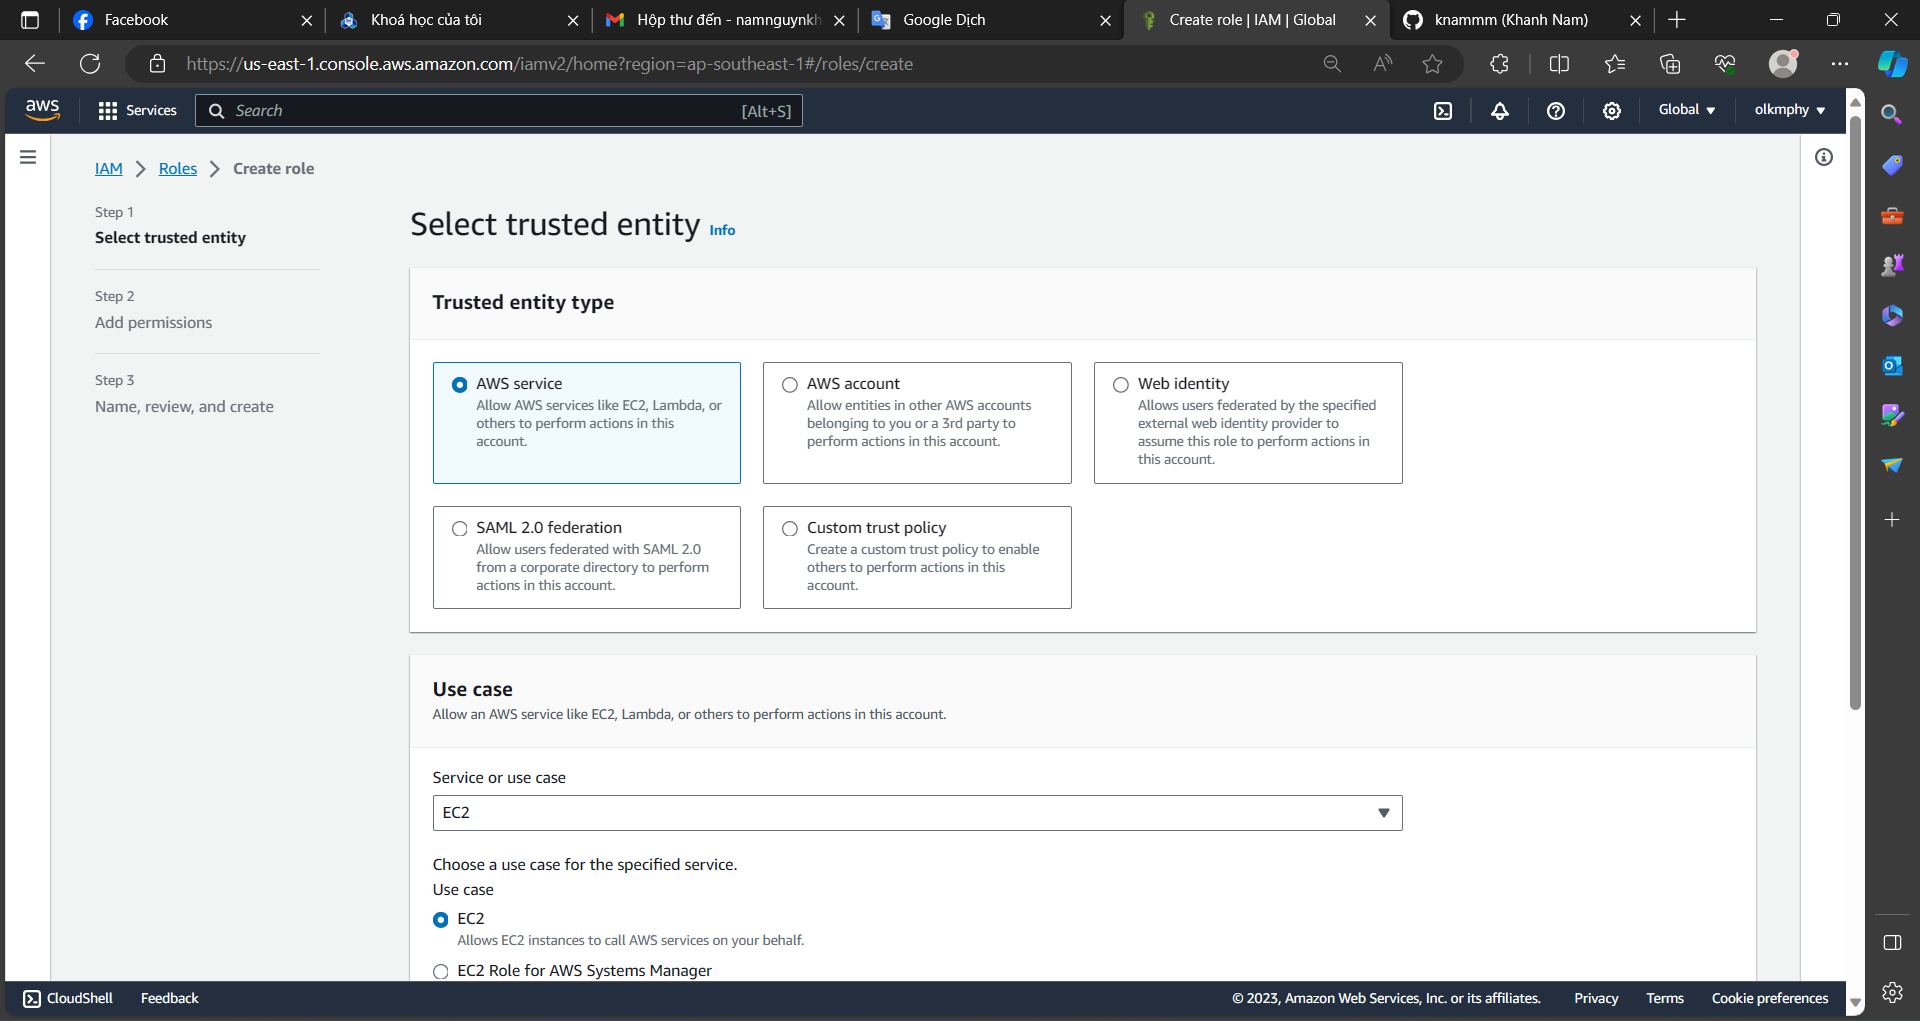
\includegraphics[width=12cm]{Pictures/Set up/IAM_Role_1.png}
    \caption{Create IAM Role for EC2 instance.}
    \label{fig:enter-label}
\end{figure}

\begin{figure}[h]
    \centering
    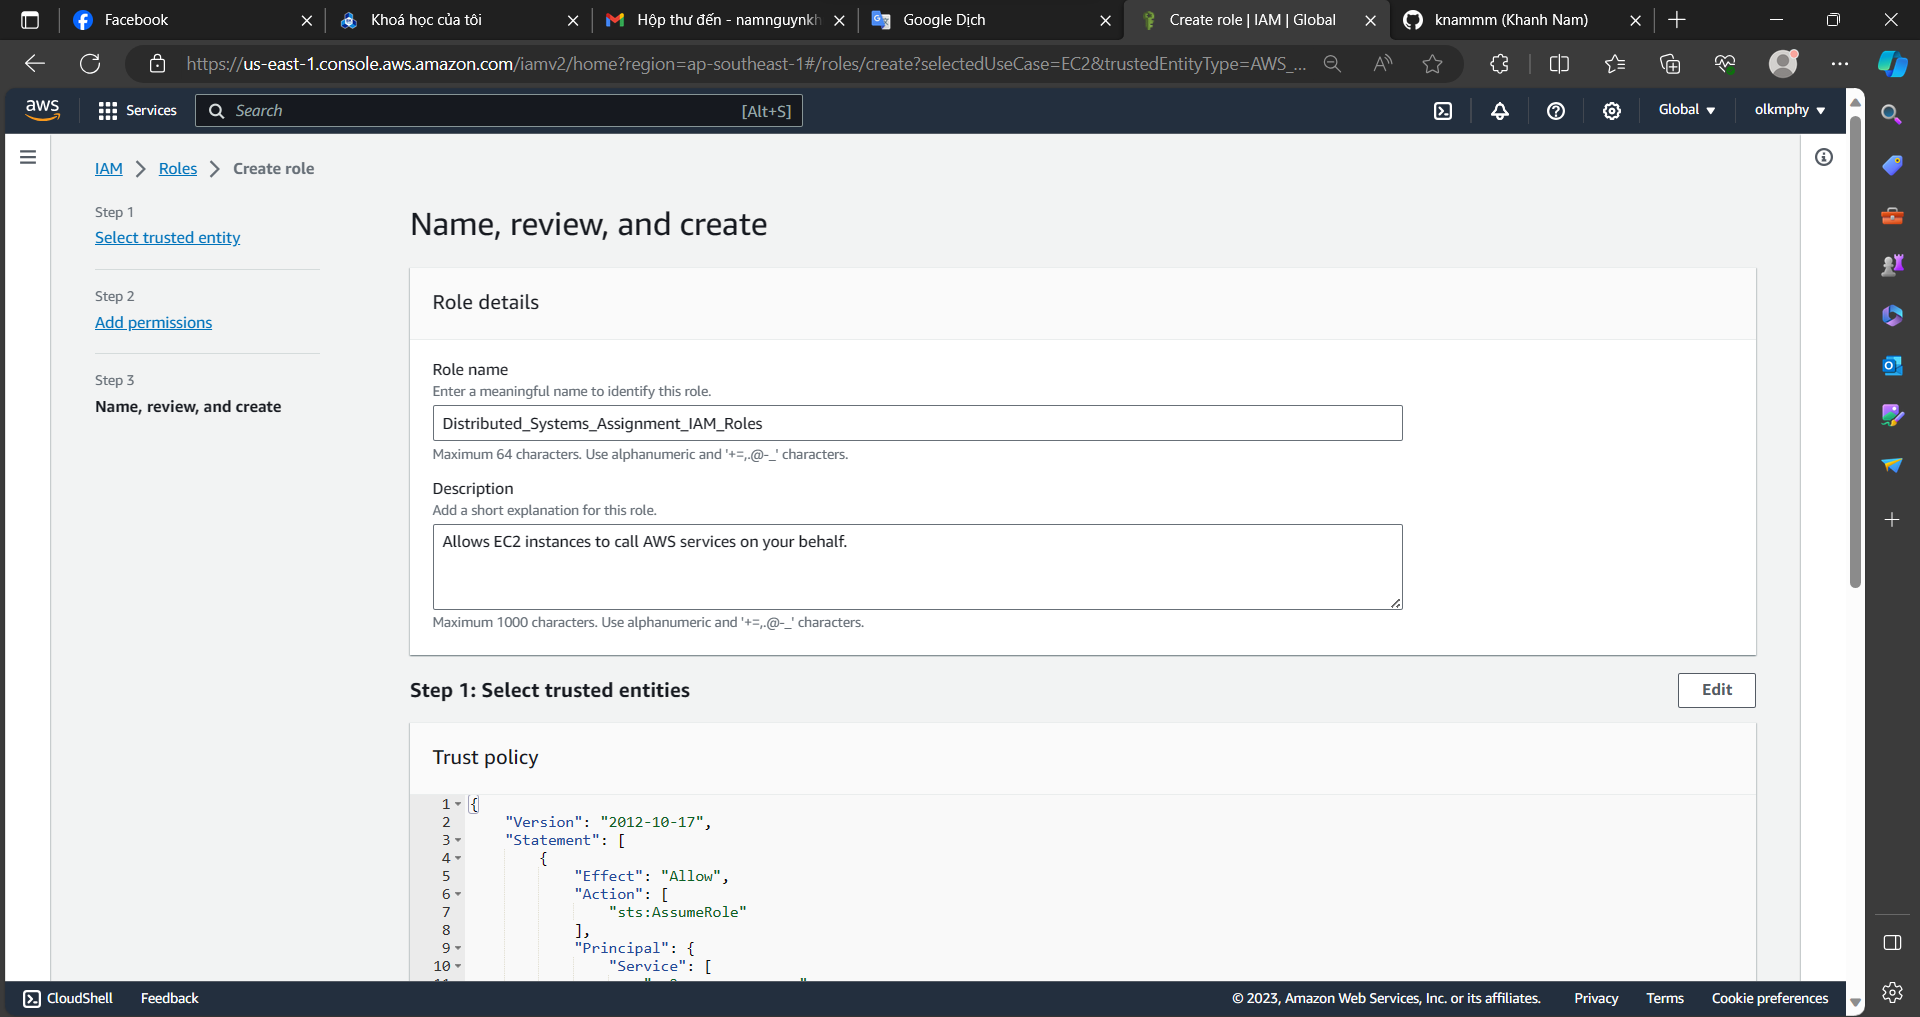
\includegraphics[width=12cm]{Pictures/Set up/IAM_Role_2.png}
    \caption{Create IAM Role for EC2 instance.}
    \label{fig:enter-label}
\end{figure}
\newpage

\begin{figure}[h]
    \centering
    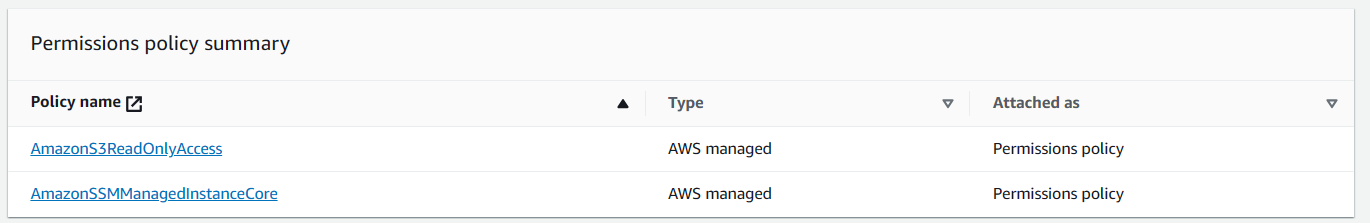
\includegraphics[width=12cm]{Pictures/Set up/IAM_Role_3.png}
    \caption{Create IAM Role for EC2 instance.}
    \label{fig:enter-label}
\end{figure}

\begin{figure}[h]
    \centering
    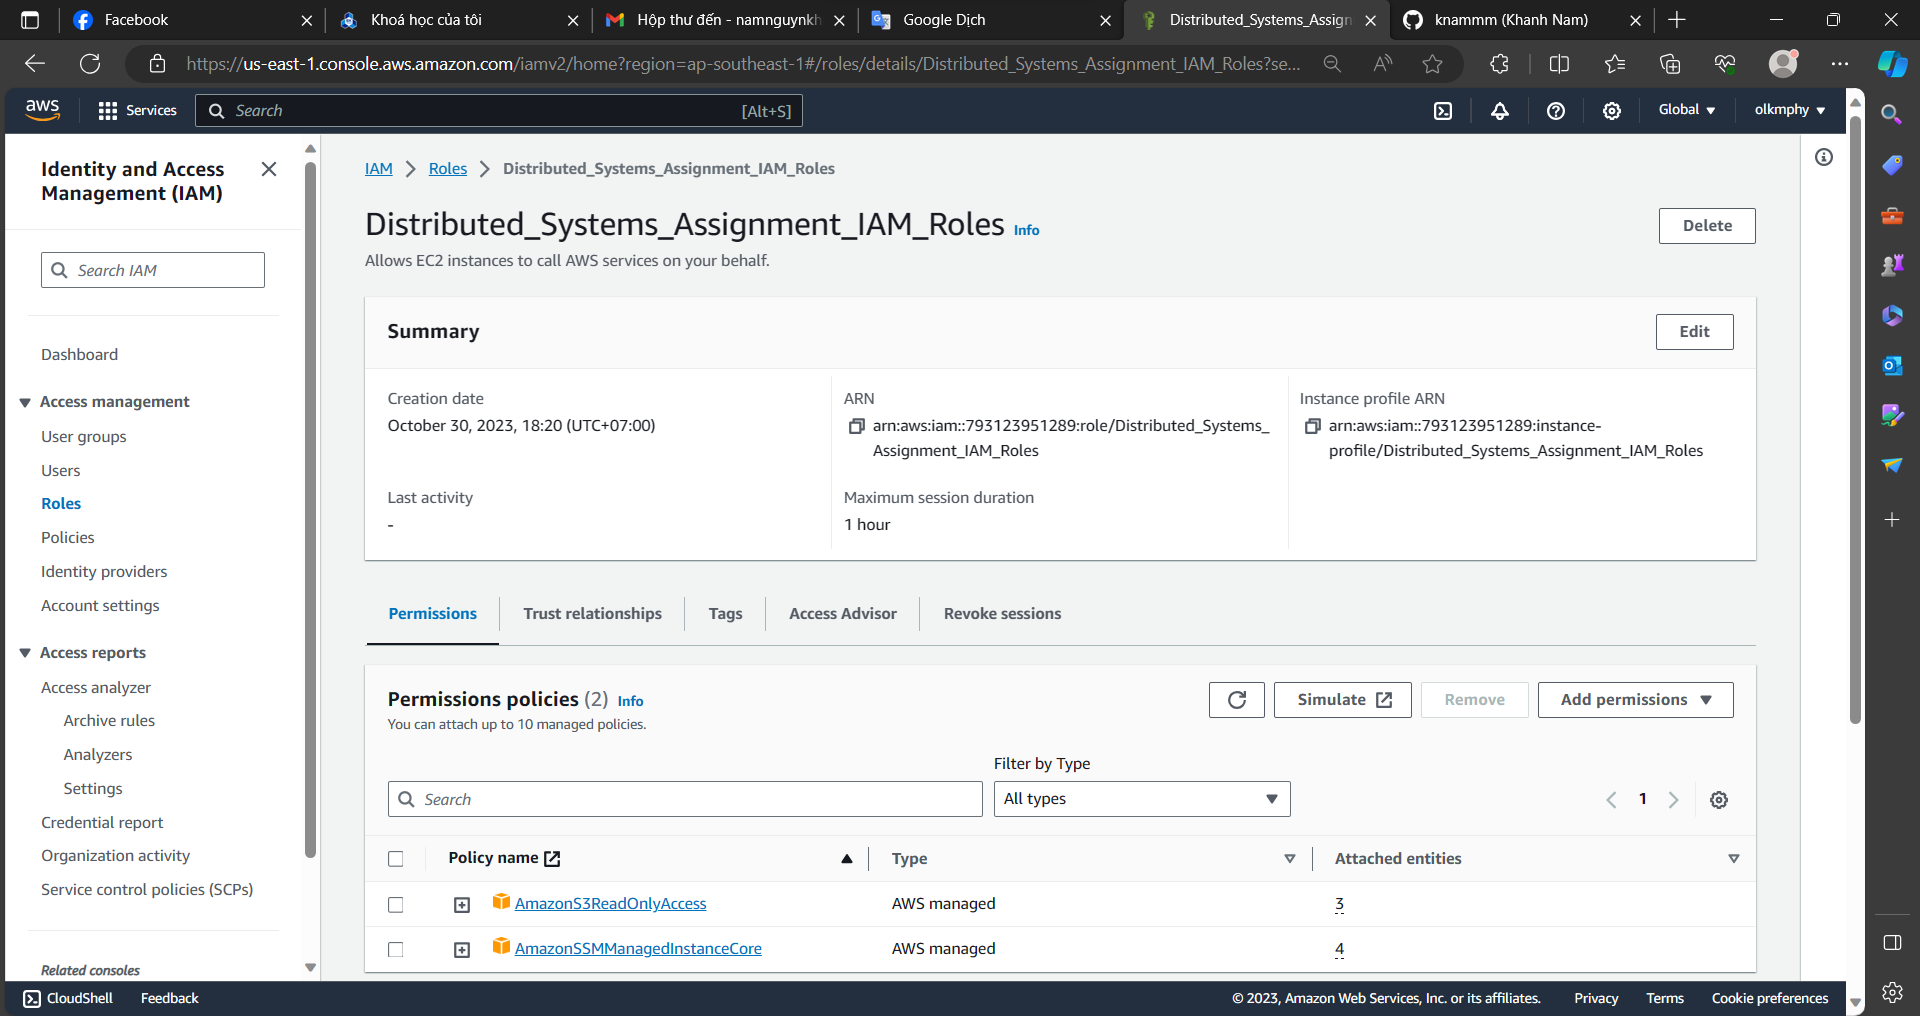
\includegraphics[width=12cm]{Pictures/Set up/IAM_Role_4.png}
    \caption{Create IAM Role for EC2 instance.}
    \label{fig:enter-label}
\end{figure}

After finishing creating bucket and IAM role, we will then continue to the next is to configure the network and sercurity.\par

\newpage
\subsection{Networking and Security}
In this section, we are going to configure the network and security for our application. We will work with Virtual Priavte Cloud, Subnets, Route Table, Internet Gateway - NAT gateway and finally the Security Groups.\par
\subsubsection{Virtual Private Cloud and Subnets}
To begin with, I will create an individual Virtual Private Cloud for this project. By navigating to the VPC dashboard in the AWS console and navigate to "Your VPCs". Here, we will select the "Create VPC" option.

\begin{figure}[h]
    \centering
    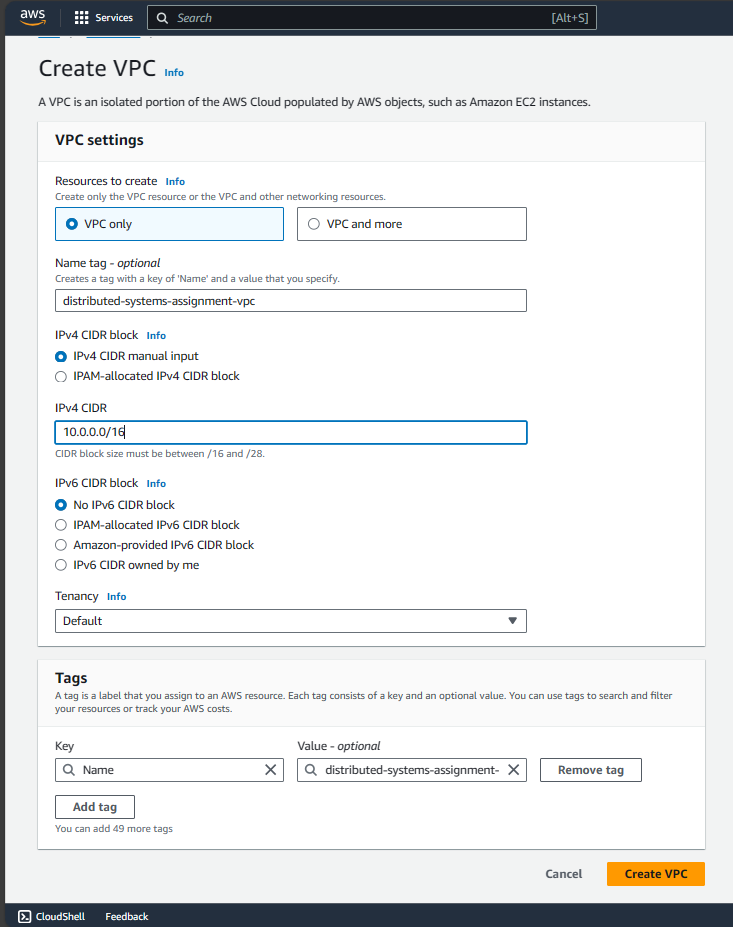
\includegraphics[width=12cm]{Pictures/Networking and Security/VPC_create.png}
    \caption{Create VPC.}
    \label{fig:enter-label}
\end{figure}
By using this specific VPC, we can deploy our application in this area. Next step is to create the Subnets in this VPC. This project will use 6 subnets including two public subnets for the web-tier and 4 private subnets for the app-tier and database.\par

\newpage
\begin{figure}[!htp]
    \centering
    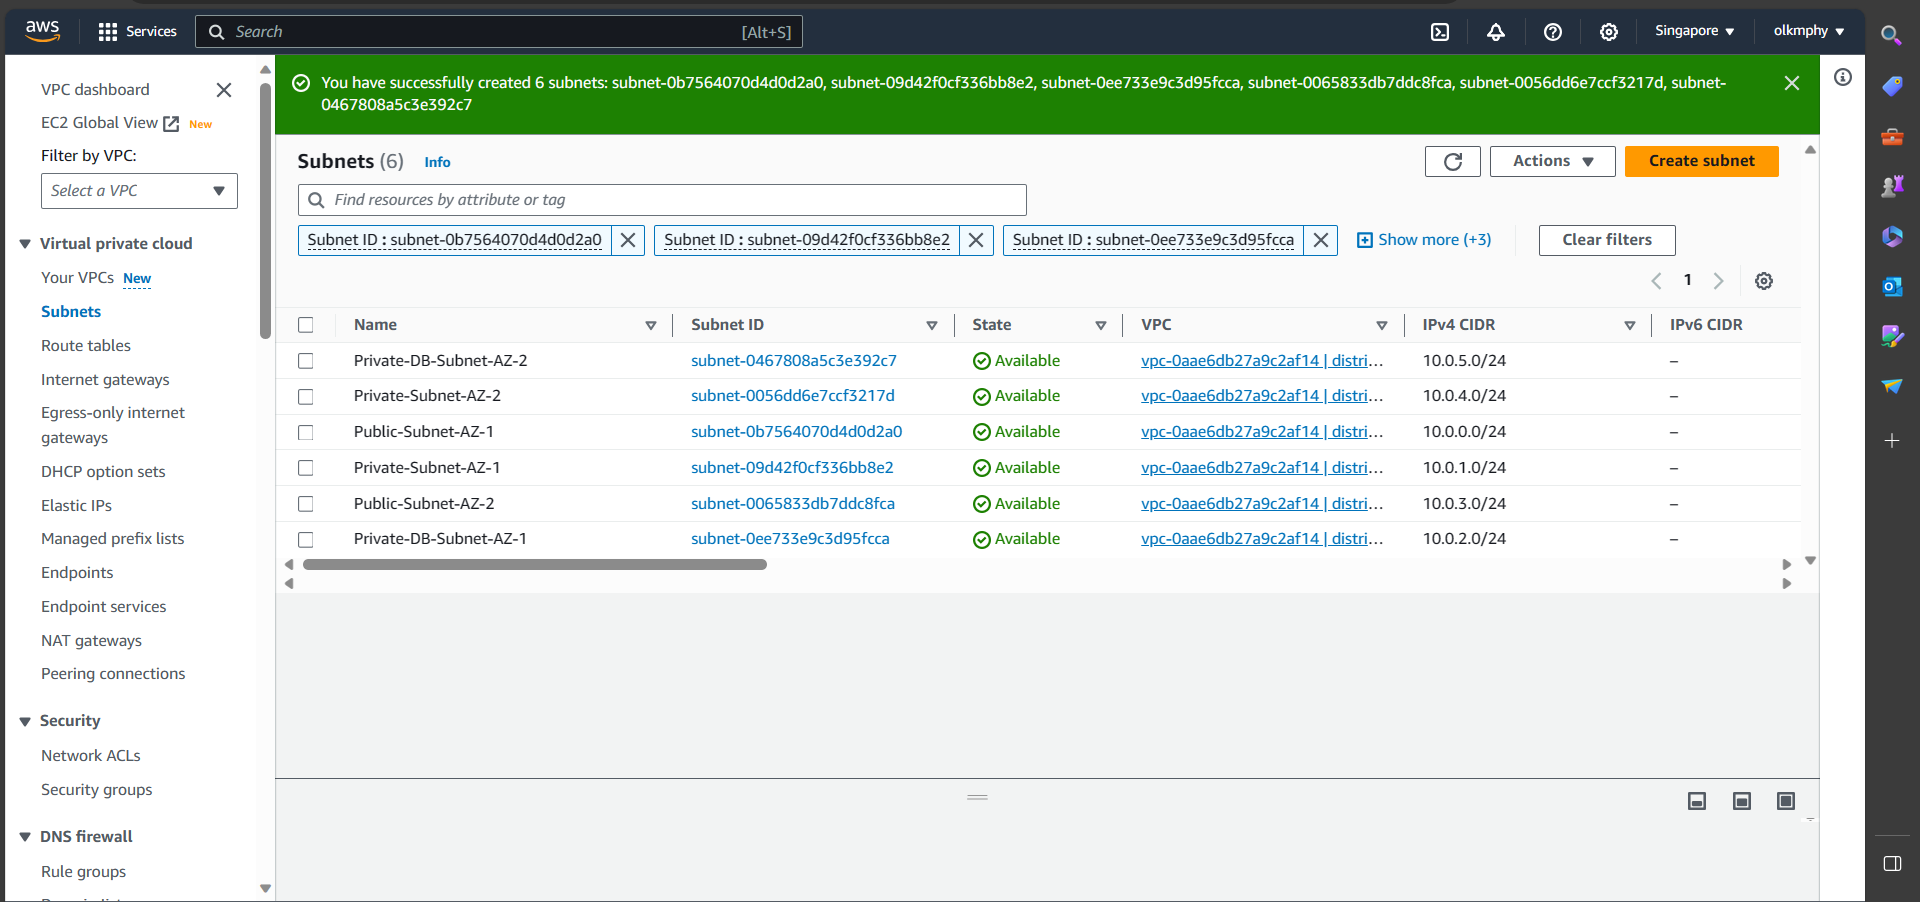
\includegraphics[width=12cm]{Pictures/Networking and Security/Subnets_create.png}
    \caption{Create Subnet.}
    \label{fig:enter-label}
\end{figure}

Next step is to configure the Internet gateway and NAT gateway for the subnets.\par
\subsubsection{Internet Connectivity}
First of all, we will set up the Internet Gateway which is attached to the VPC that I have created before so that when there is a connection which is outside of the VPC, it will communicate with this gateway. Secondly, in order for our instances in the private subnet (app-tier) to be able to access the internet they will need to go through a NAT Gateway. For high availability, I will deploy one NAT gateway in each of the public subnets.\par\
\begin{figure}[h]
    \centering
    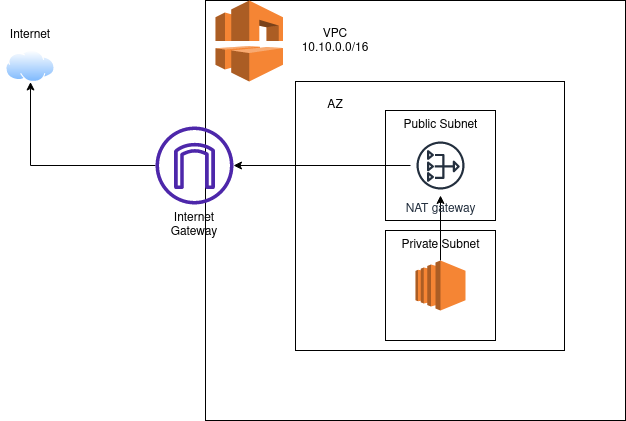
\includegraphics[width=12cm]{Pictures/Networking and Security/IGW and NAT.png}
    \caption{Internet Gateway and NAT Gateway.}
    \label{fig:enter-label}
\end{figure}

Navigating to the Internet gateways in VPC section to create our gateways.\par

\begin{figure}[h]
    \centering
    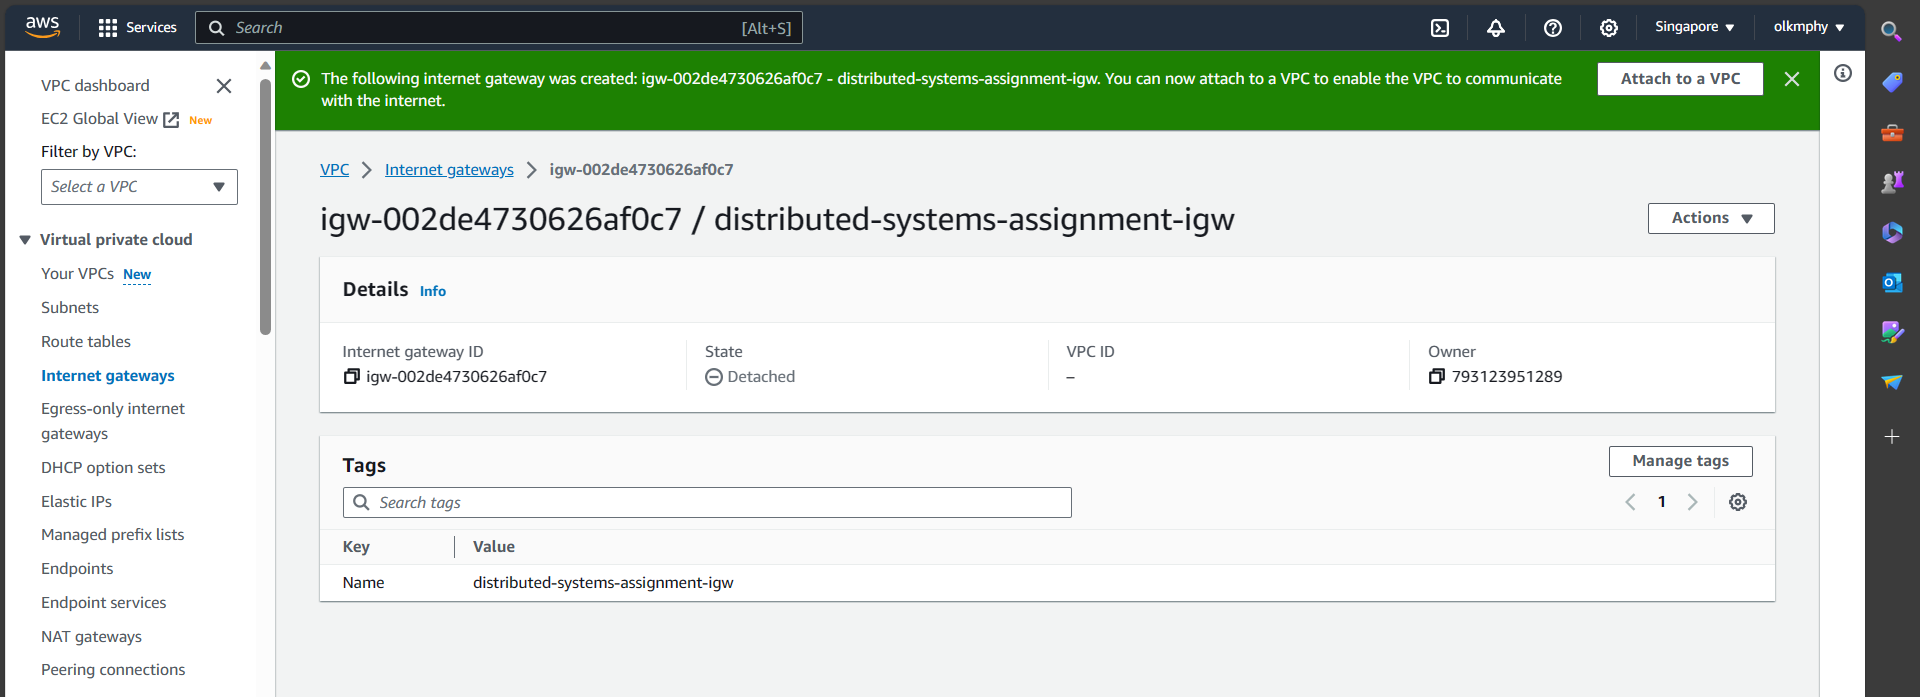
\includegraphics[width=12cm]{Pictures/Networking and Security/igw_create.png}
    \caption{Create an internet gateway.}
    \label{fig:enter-label}
\end{figure}

\begin{figure}[h]
    \centering
    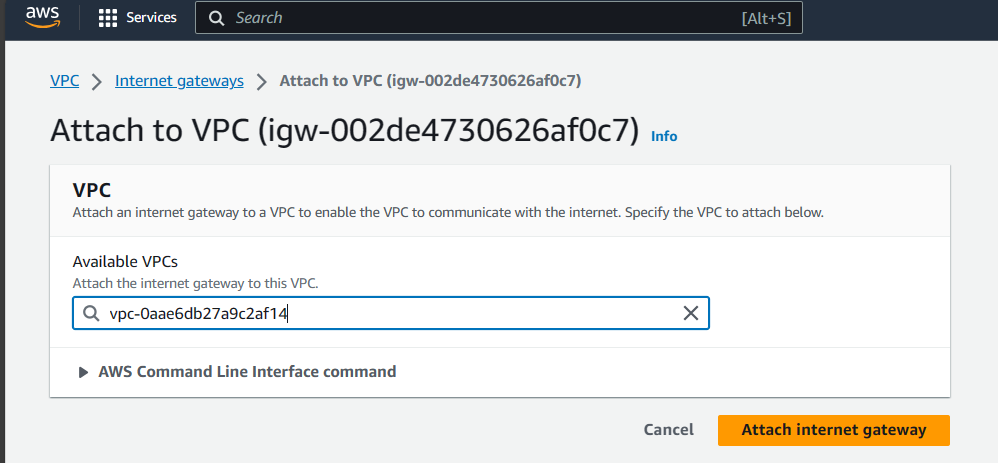
\includegraphics[width=12cm]{Pictures/Networking and Security/igw_attach.png}
    \caption{Attach the internet gateway to the VPC.}
    \label{fig:enter-label}
\end{figure}

\newpage
Then continually create two NAT gateways and attach each of them to each of the public subnets.\par

\begin{figure}[!htp]
    \centering
    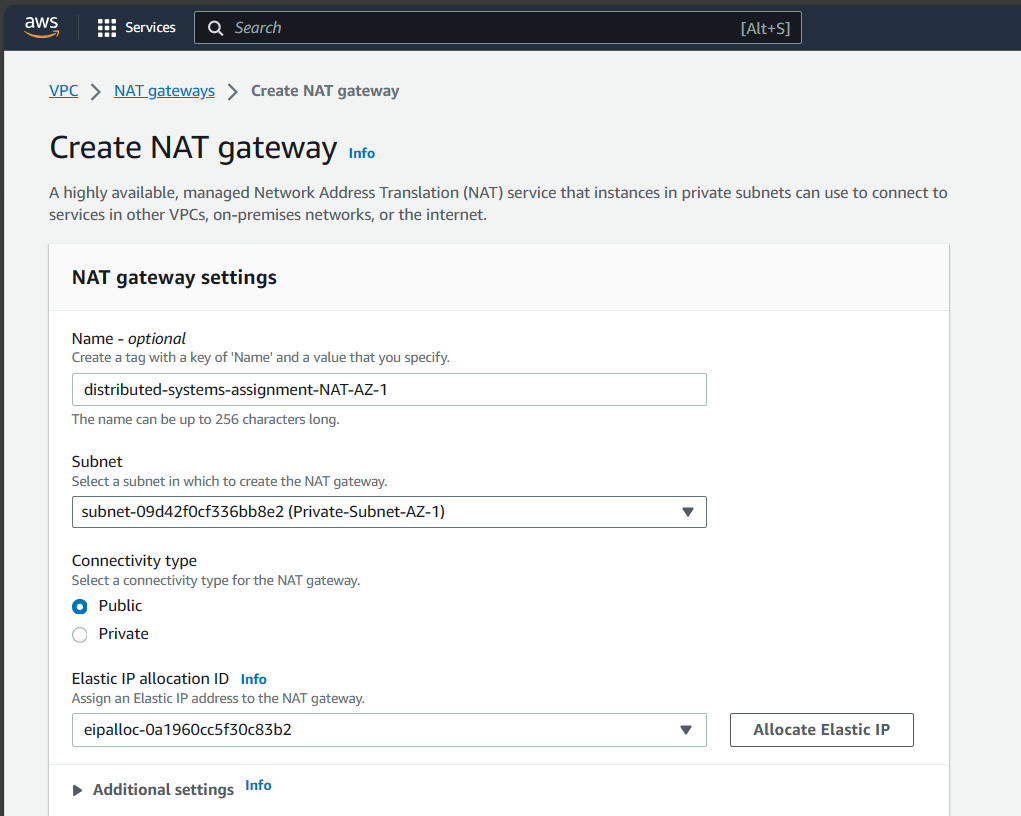
\includegraphics[width=12cm]{Pictures/Networking and Security/NAT_create_1.png}
    \caption{Create the first NAT at AZ-1.}
    \label{fig:enter-label}
\end{figure}

\newpage
\begin{figure}[h]
    \centering
    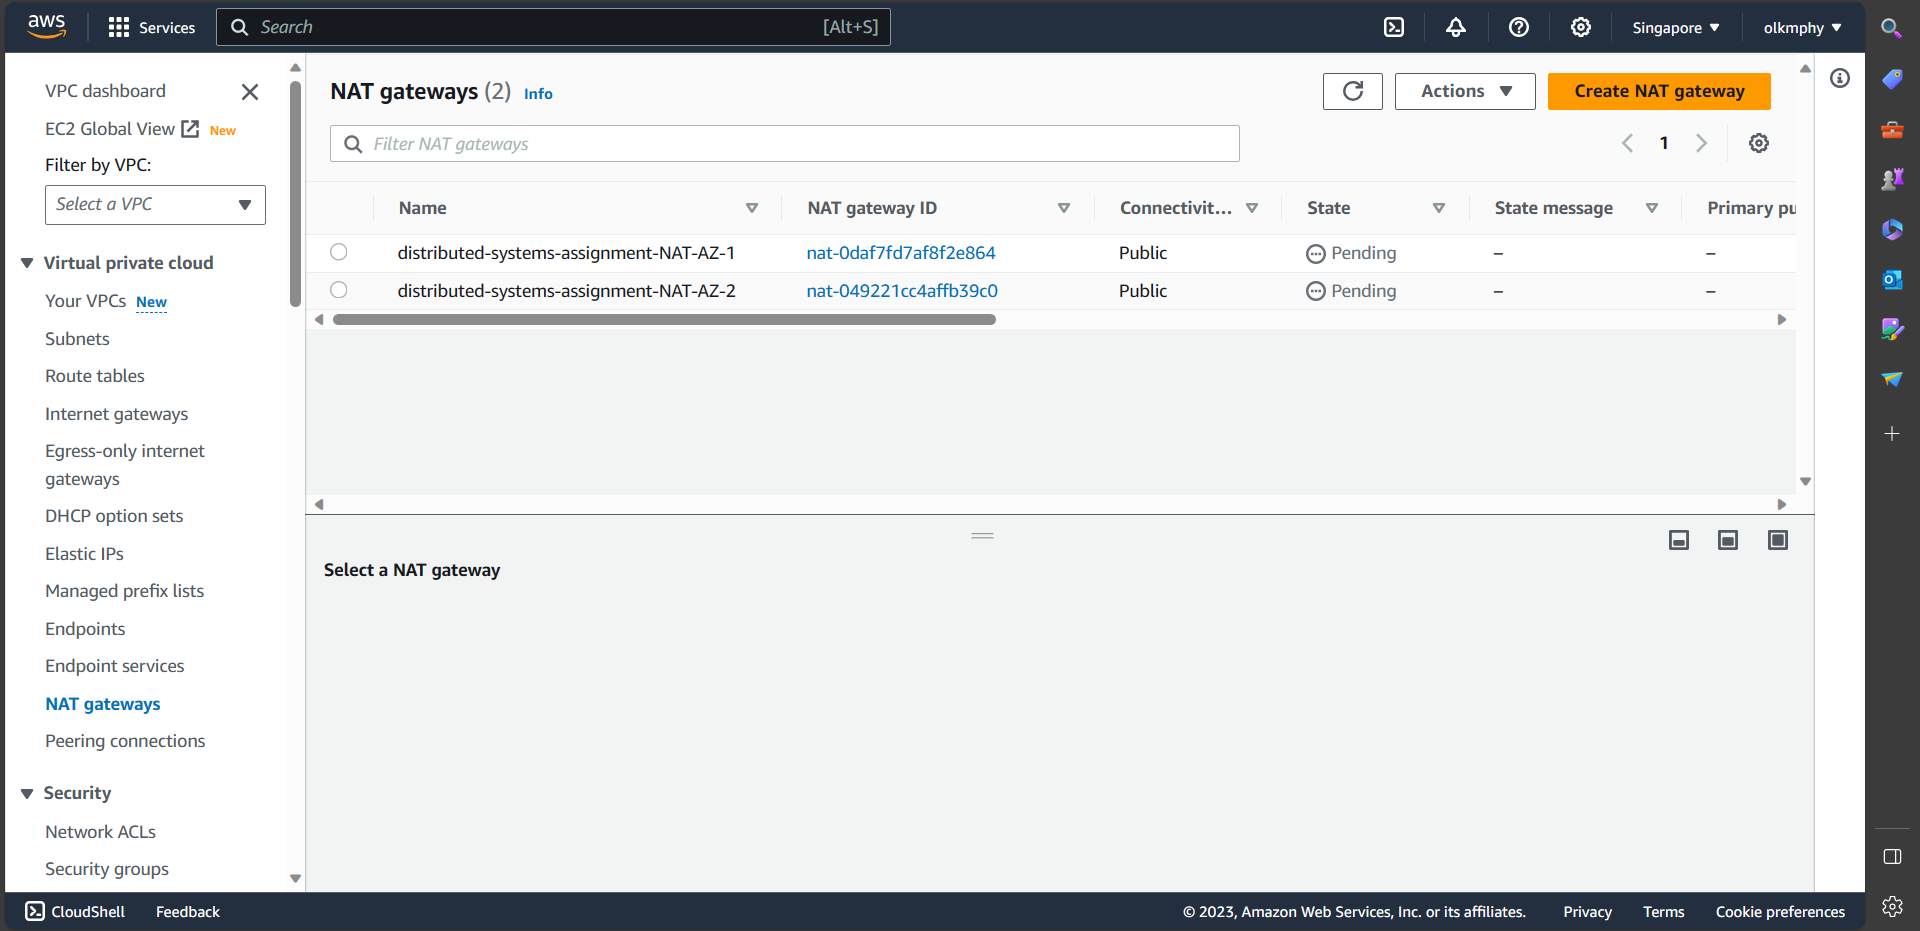
\includegraphics[width=12cm]{Pictures/Networking and Security/NAT_create_2.png}
    \caption{Create the second NAT at AZ-2.}
    \label{fig:enter-label}
\end{figure}

After finishing the configuration of the internet connectivity, we will then continue to move to the routing configuration.

\subsubsection{Routing Configuration}
In AWS, we will use the Route Table to control the connectivity in our VPC. In this section, we will create 3 route tables. One of them will be use for routing the connections to the public subnets.\par

\begin{figure}[h]
    \centering
    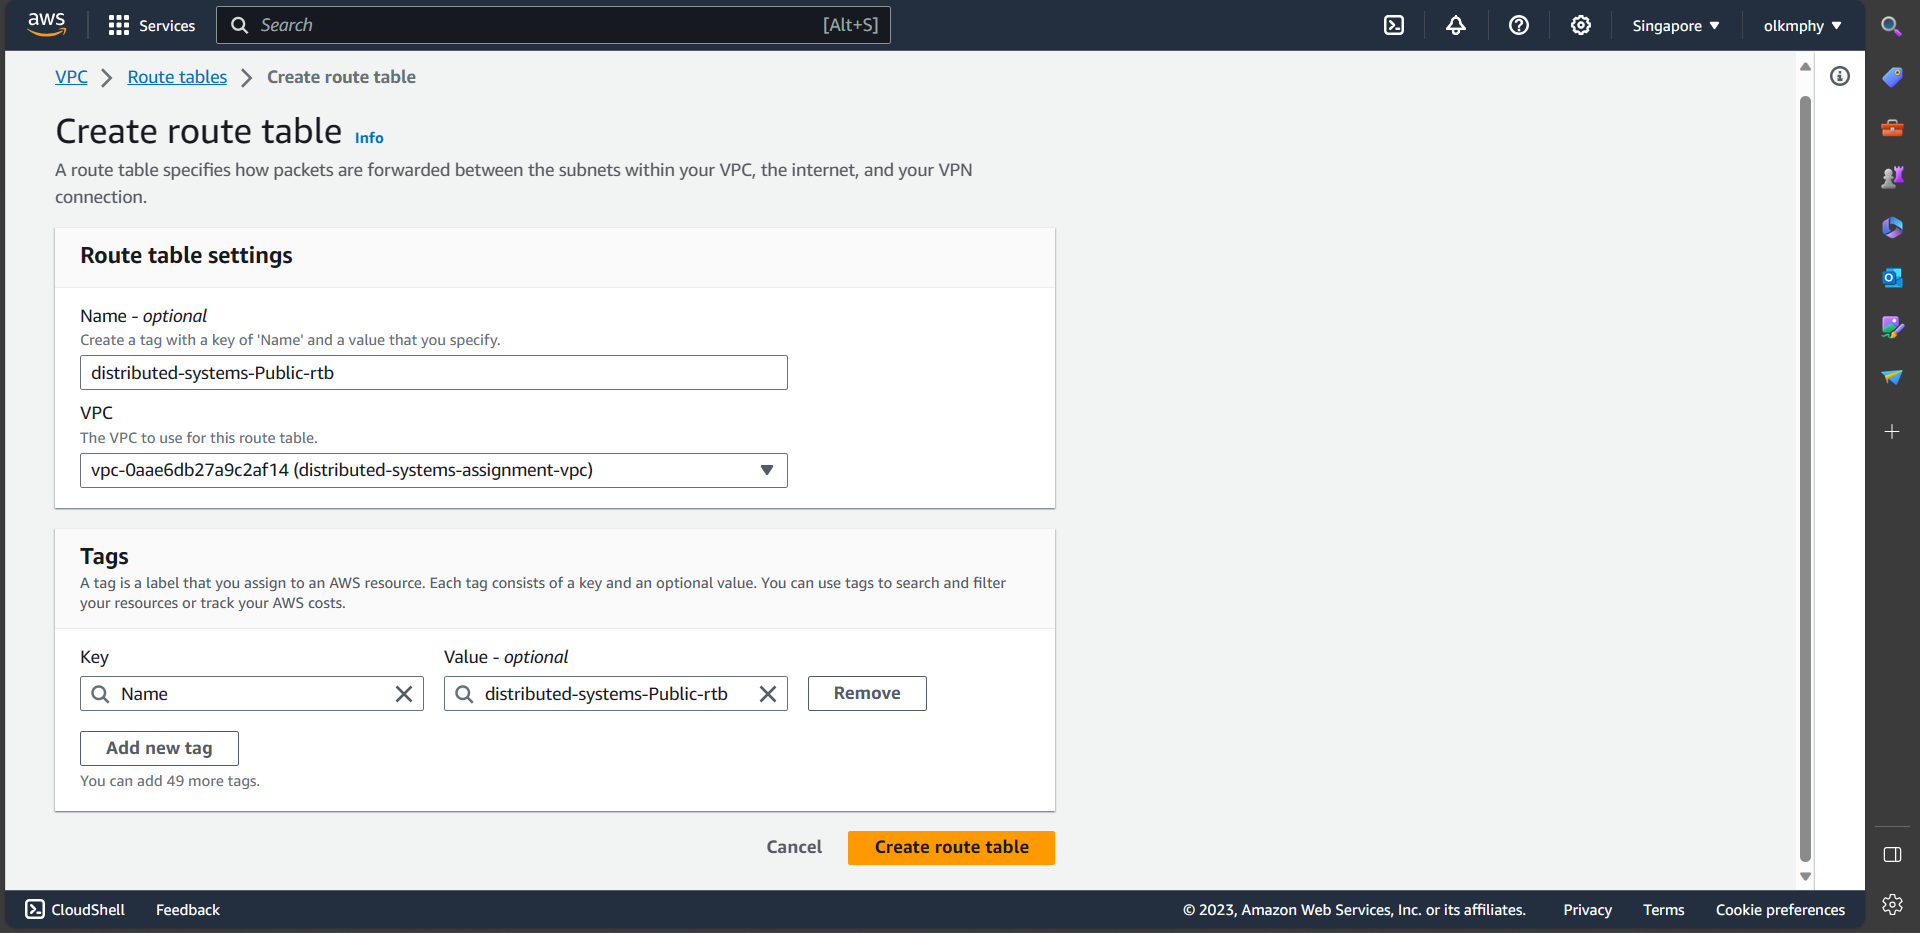
\includegraphics[width=10cm]{Pictures/Networking and Security/route_table_create.png}
    \caption{Create a Route Table.}
    \label{fig:enter-label}
\end{figure}

Then, add a route that directs traffic from the VPC to the internet gateway. In other words, for all traffic destined for IPs outside the VPC CDIR range, add an entry that directs it to the internet gateway as a target.\par

\begin{figure}[h]
    \centering
    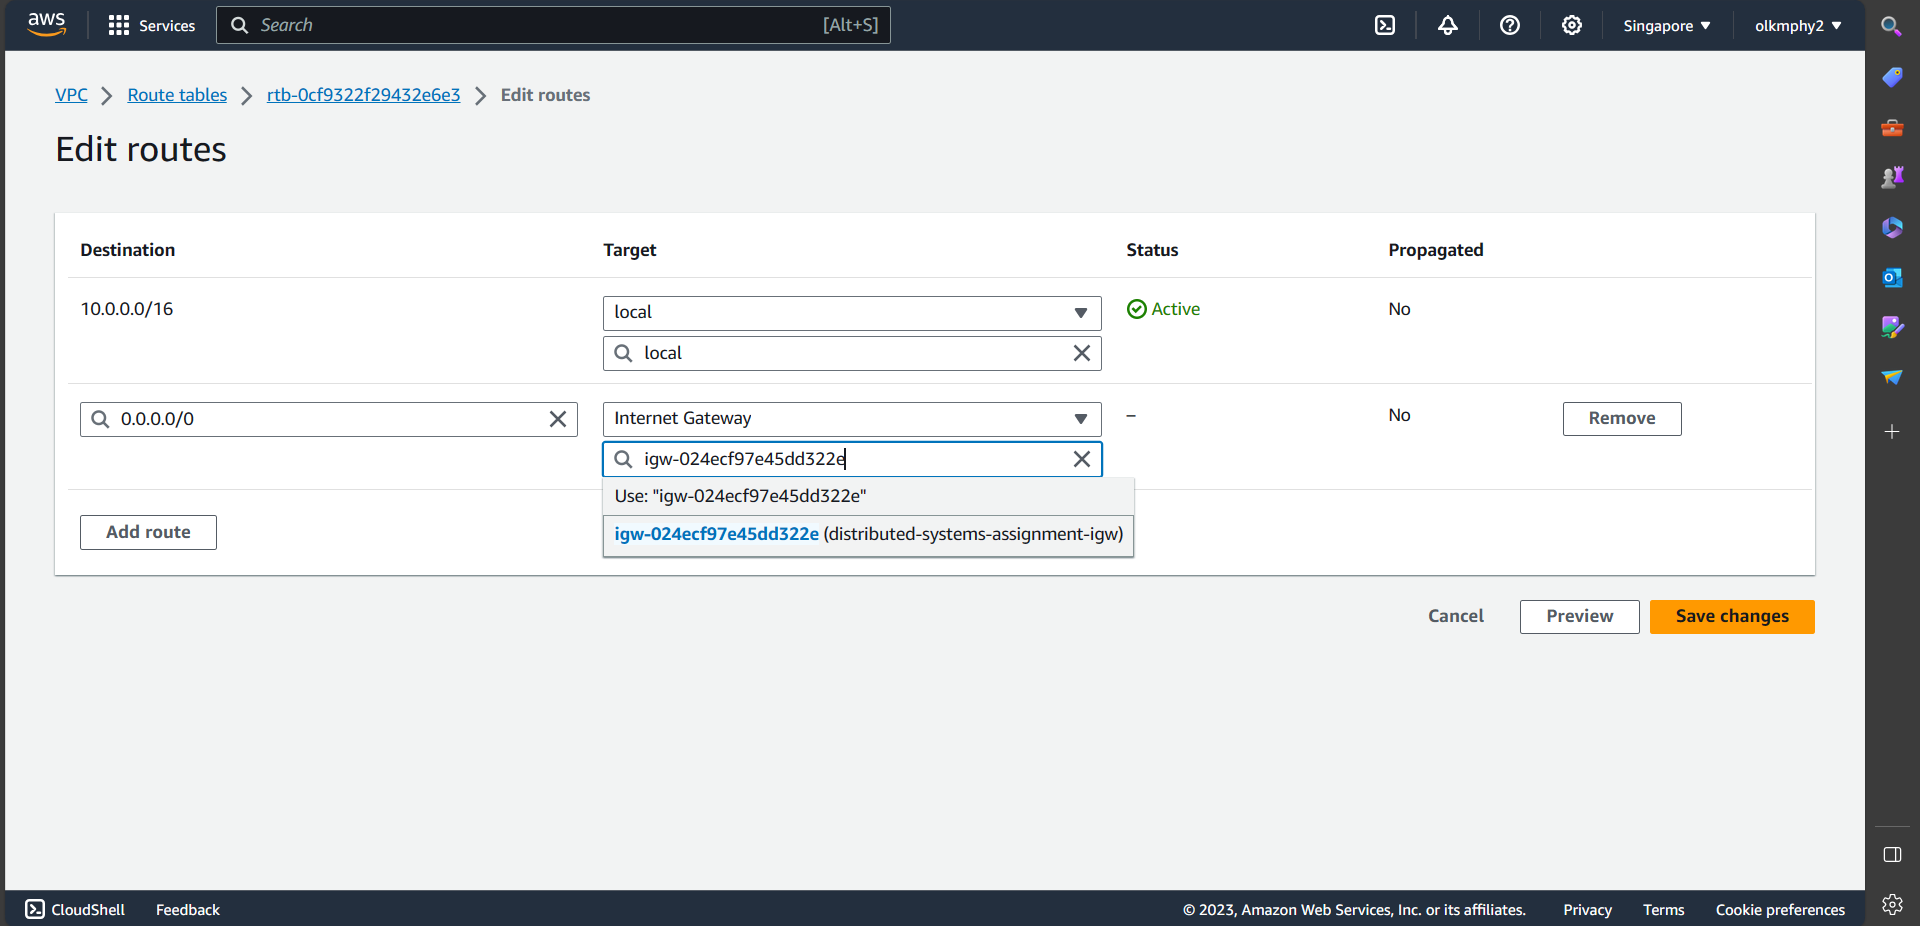
\includegraphics[width=10cm]{Pictures/Networking and Security/Edit_route_public.png}
    \caption{Add route from outside VPC.}
    \label{fig:enter-label}
\end{figure}

\newpage
Next, we will associate two public subnets to this route table so that every connection to VPC will route to these two subnets.

\begin{figure}[!htp]
    \centering
    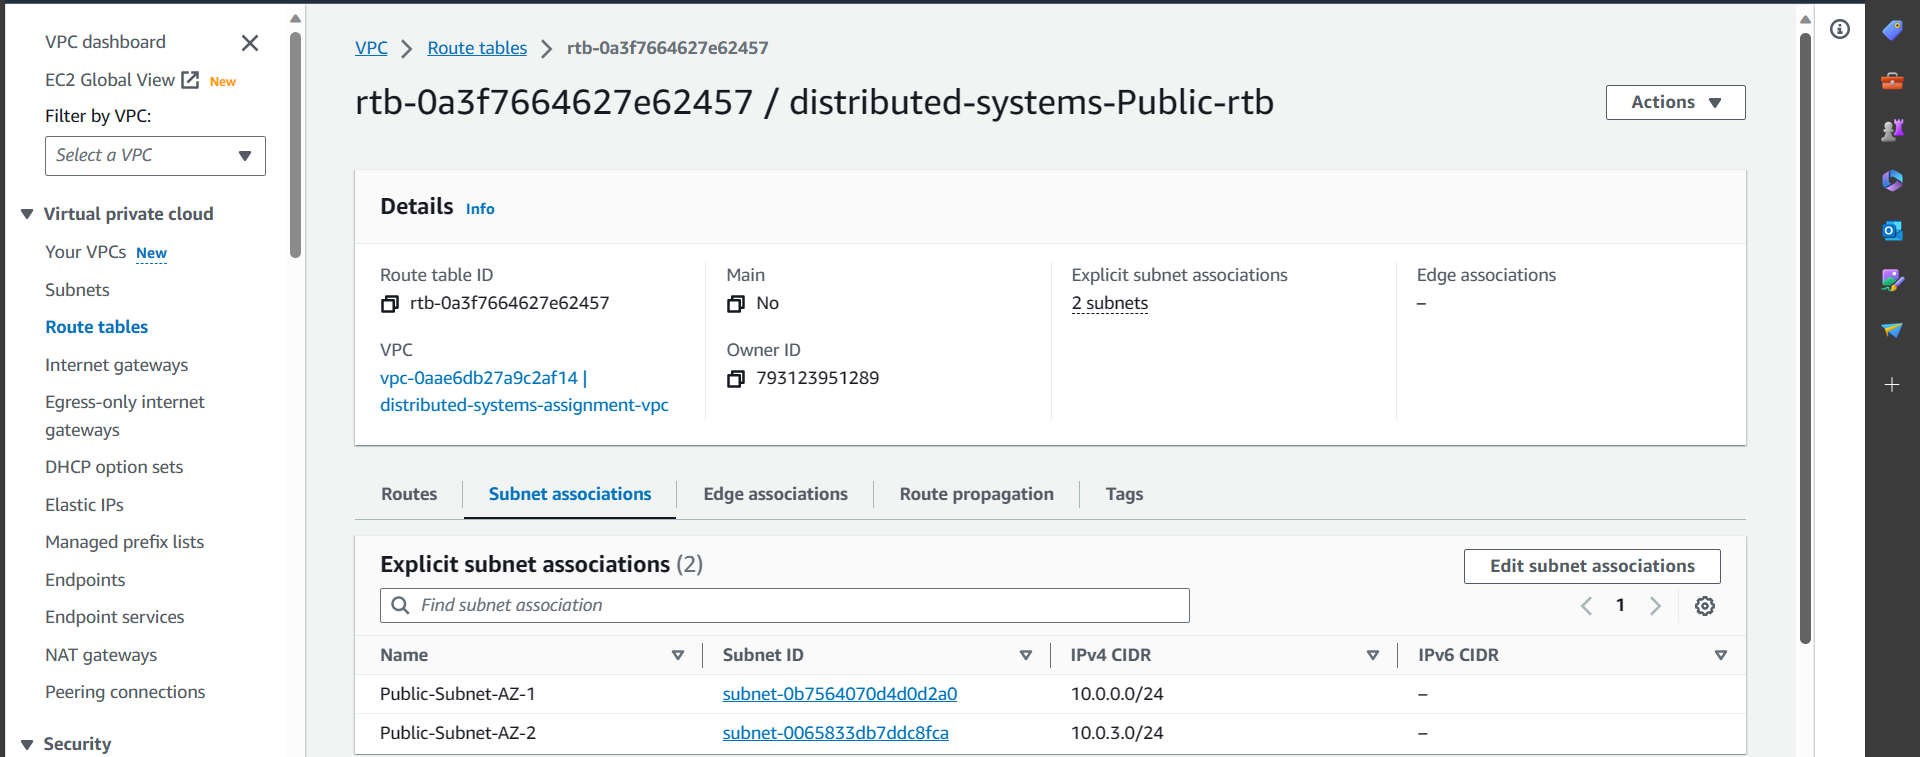
\includegraphics[width=12cm]{Pictures/Networking and Security/Public_rtb_Sub_Asso.png}
    \caption{Edit subnet associations.}
    \label{fig:enter-label}
\end{figure}

Now we will create 2 more route tables, one for each is an app-layer private subnet in each availability zone. These route tables will route app-layer traffic destined for outside the VPC to the NAT gateway in the respective availability zone, so add the appropriate routes for that. Once the route tables are created and routes added, add the appropriate subnet associations for each of the app layer private subnets. After all, we will have the following result.\par
\begin{figure}[h]
    \centering
    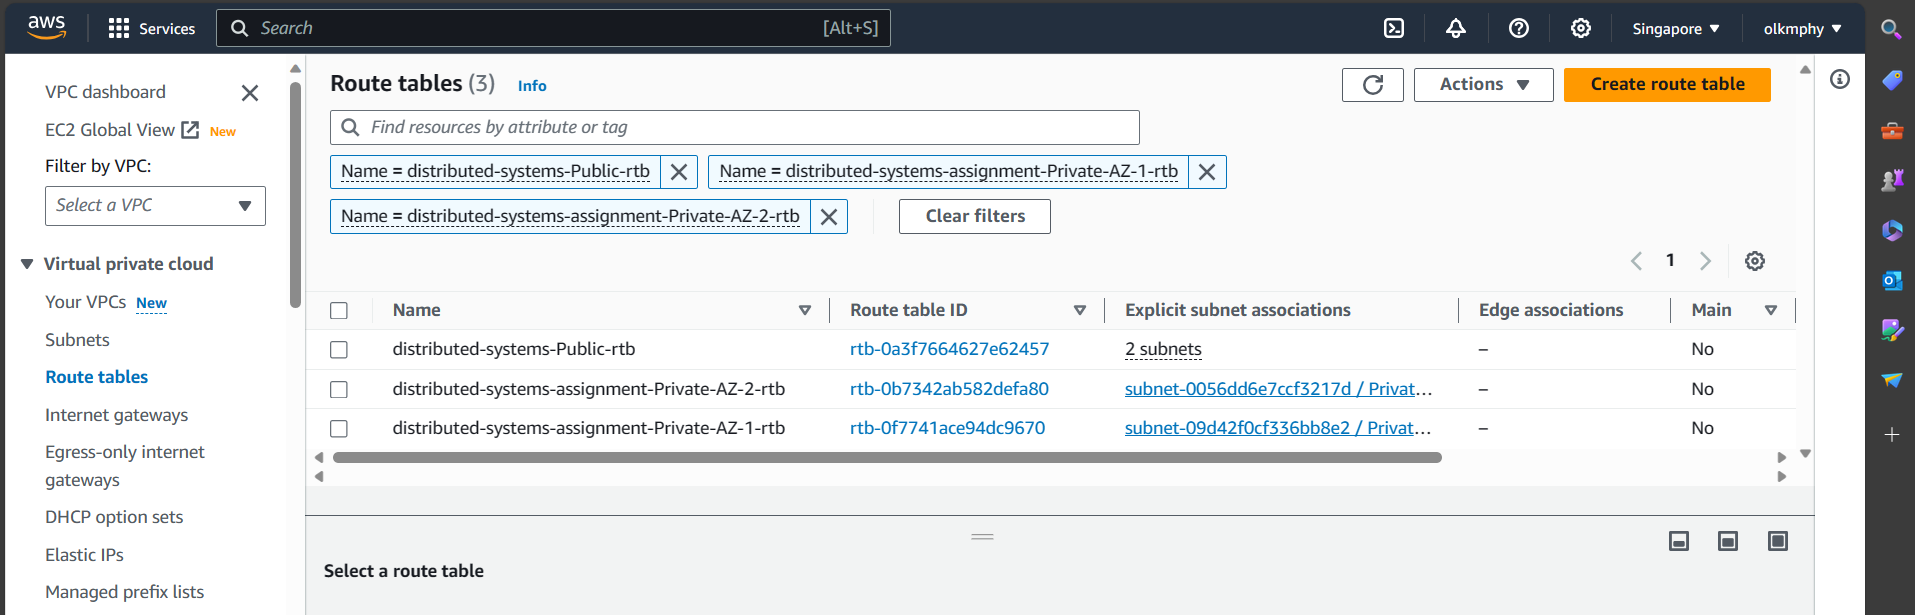
\includegraphics[width=12cm]{Pictures/Networking and Security/route_table_create_all.png}
    \caption{Three route tables.}
    \label{fig:enter-label}
\end{figure}

Now, we will move to the next section is to create the Security Groups (firewall) for future use. In this project, I will create 5 security groups for the instances, database and the load balancers.

\subsubsection{Security Groups}
The first security group that we  will create is the security group for the internet facing load balancer. We will add an inbound rule to allow HTTP type traffic for my own IP.\par
\begin{figure}[h]
    \centering
    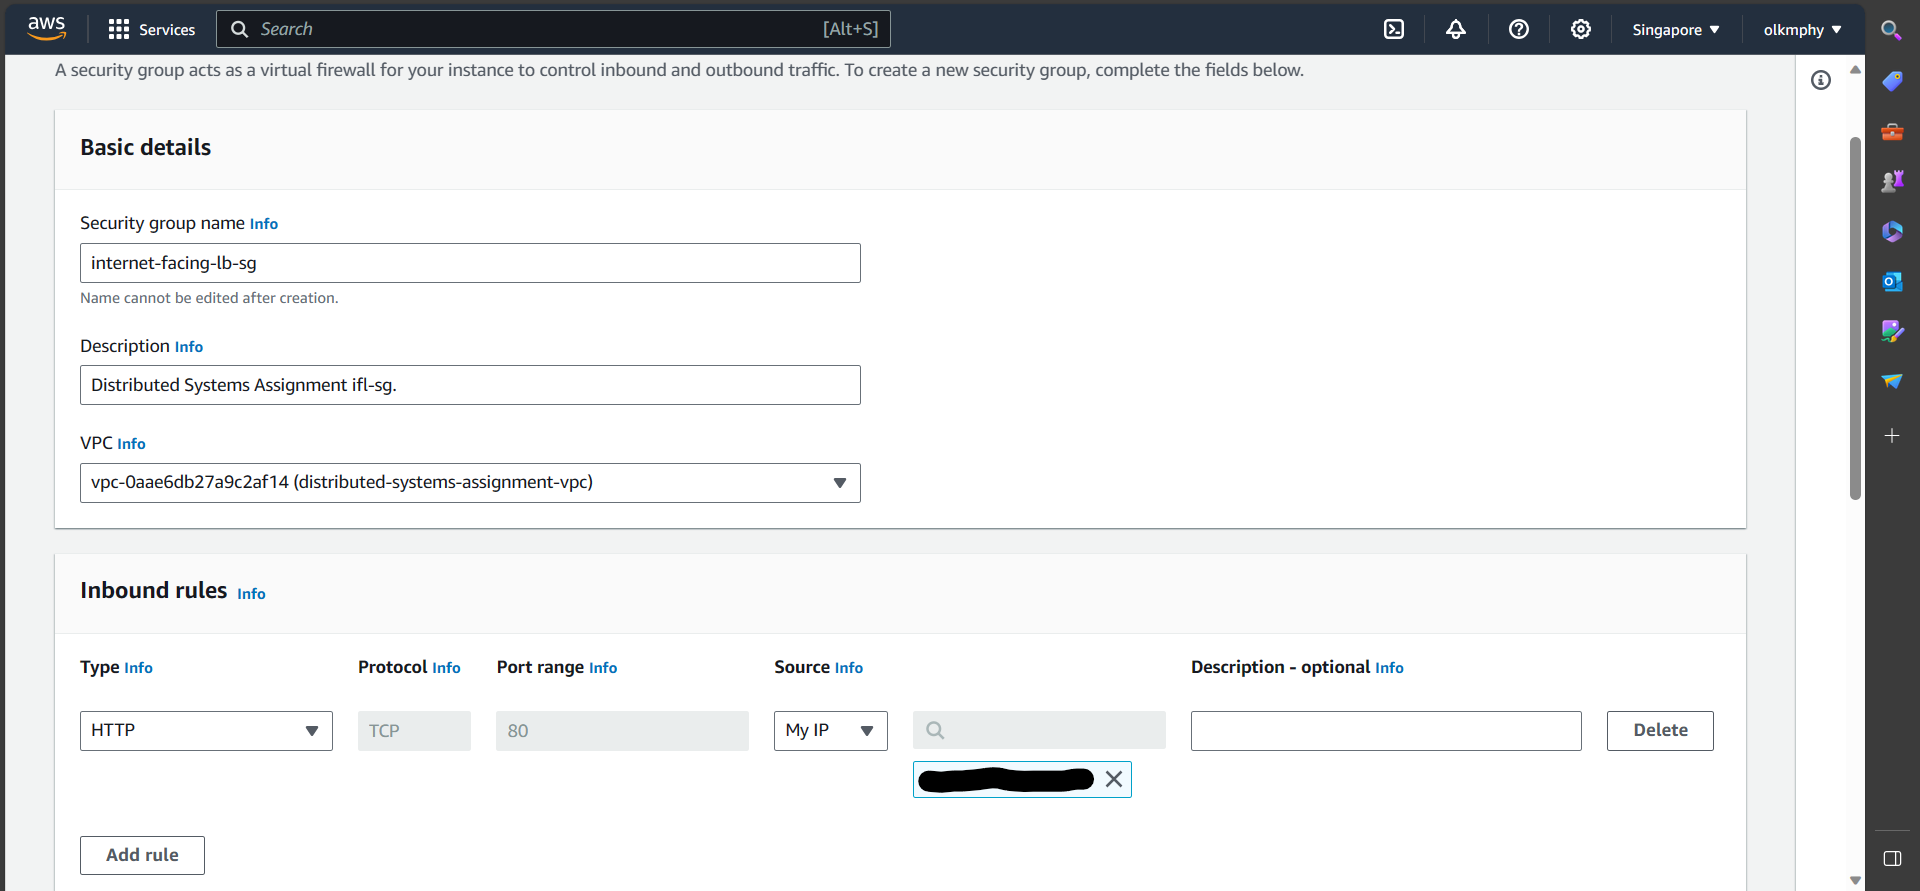
\includegraphics[width=10cm]{Pictures/Networking and Security/SG_create_1.png}
    \caption{Internet facing load balancer SG.}
    \label{fig:enter-label}
\end{figure}
\newpage

The second one will be for the web-tier instance. This will allow the traffic from my IP and also from the internet facing load balancer that we created before.\par
\begin{figure}[h]
    \centering
    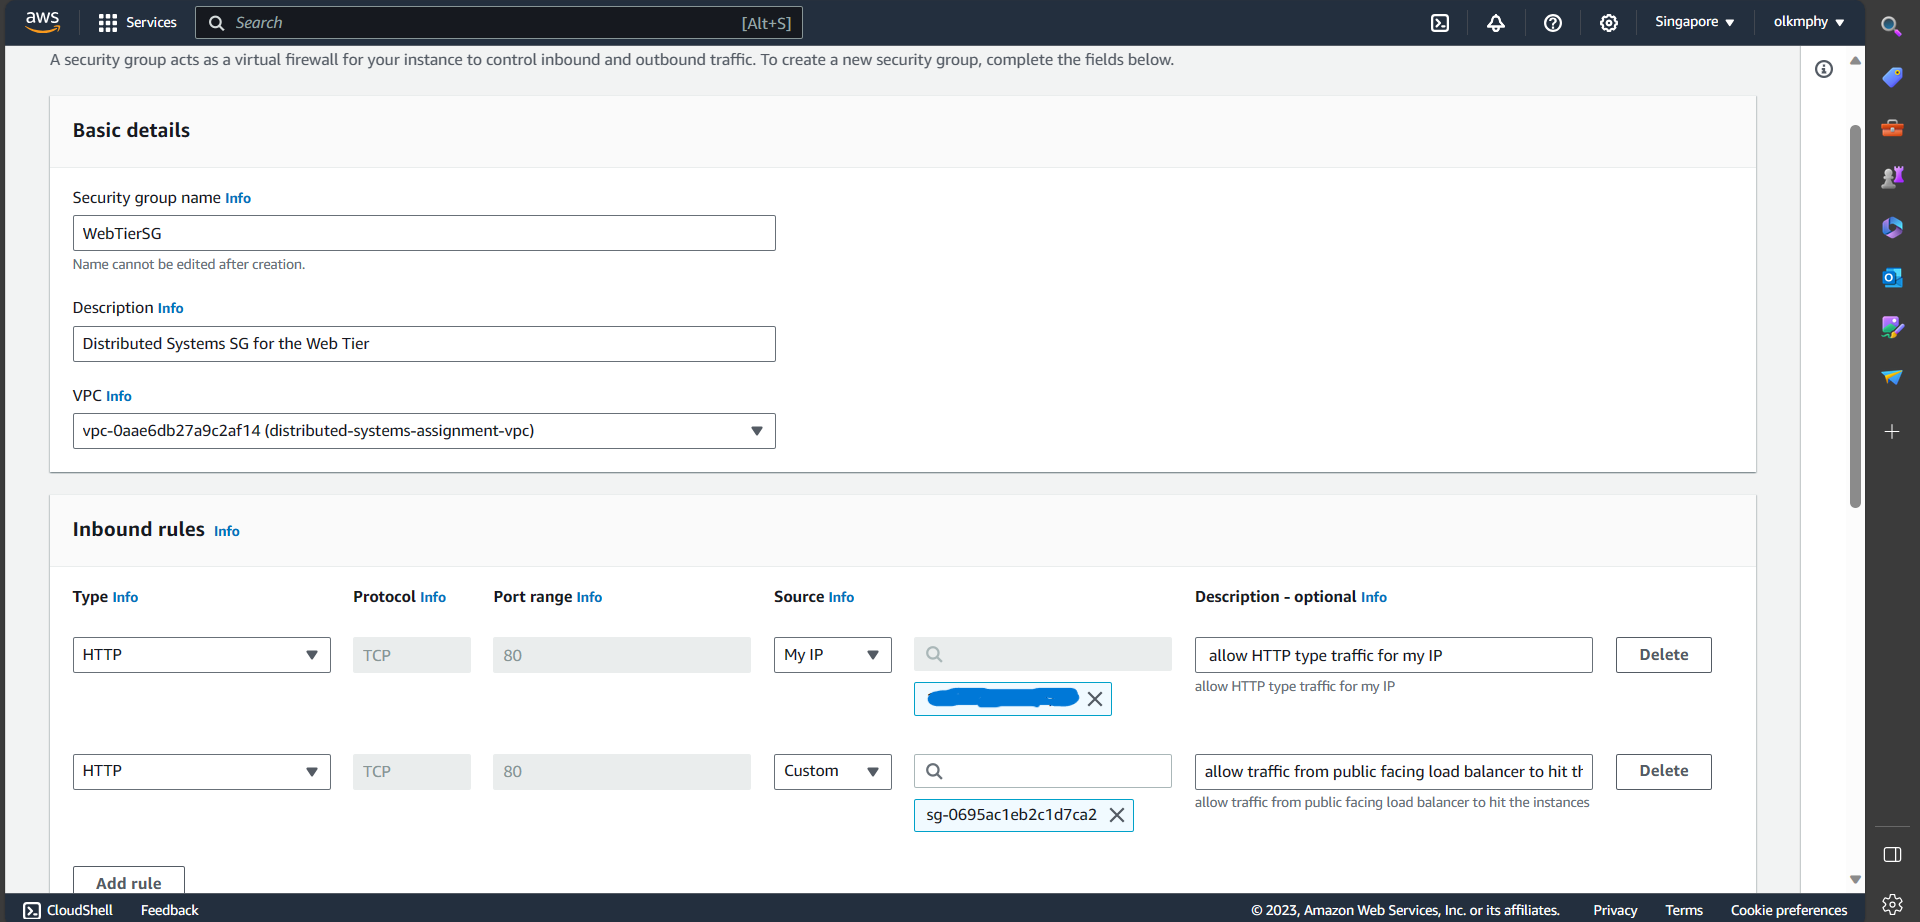
\includegraphics[width=12cm]{Pictures/Networking and Security/SG_create_2.png}
    \caption{Security Group for web-tier instances.}
    \label{fig:enter-label}
\end{figure}

The third security group that we need to deal with is the security group for the internal load balancer. And this security group allows traffic from the web-tier instance to hit the internal load balancer. The picture below will demonstrate the idea.\par

\begin{figure}[h]
    \centering
    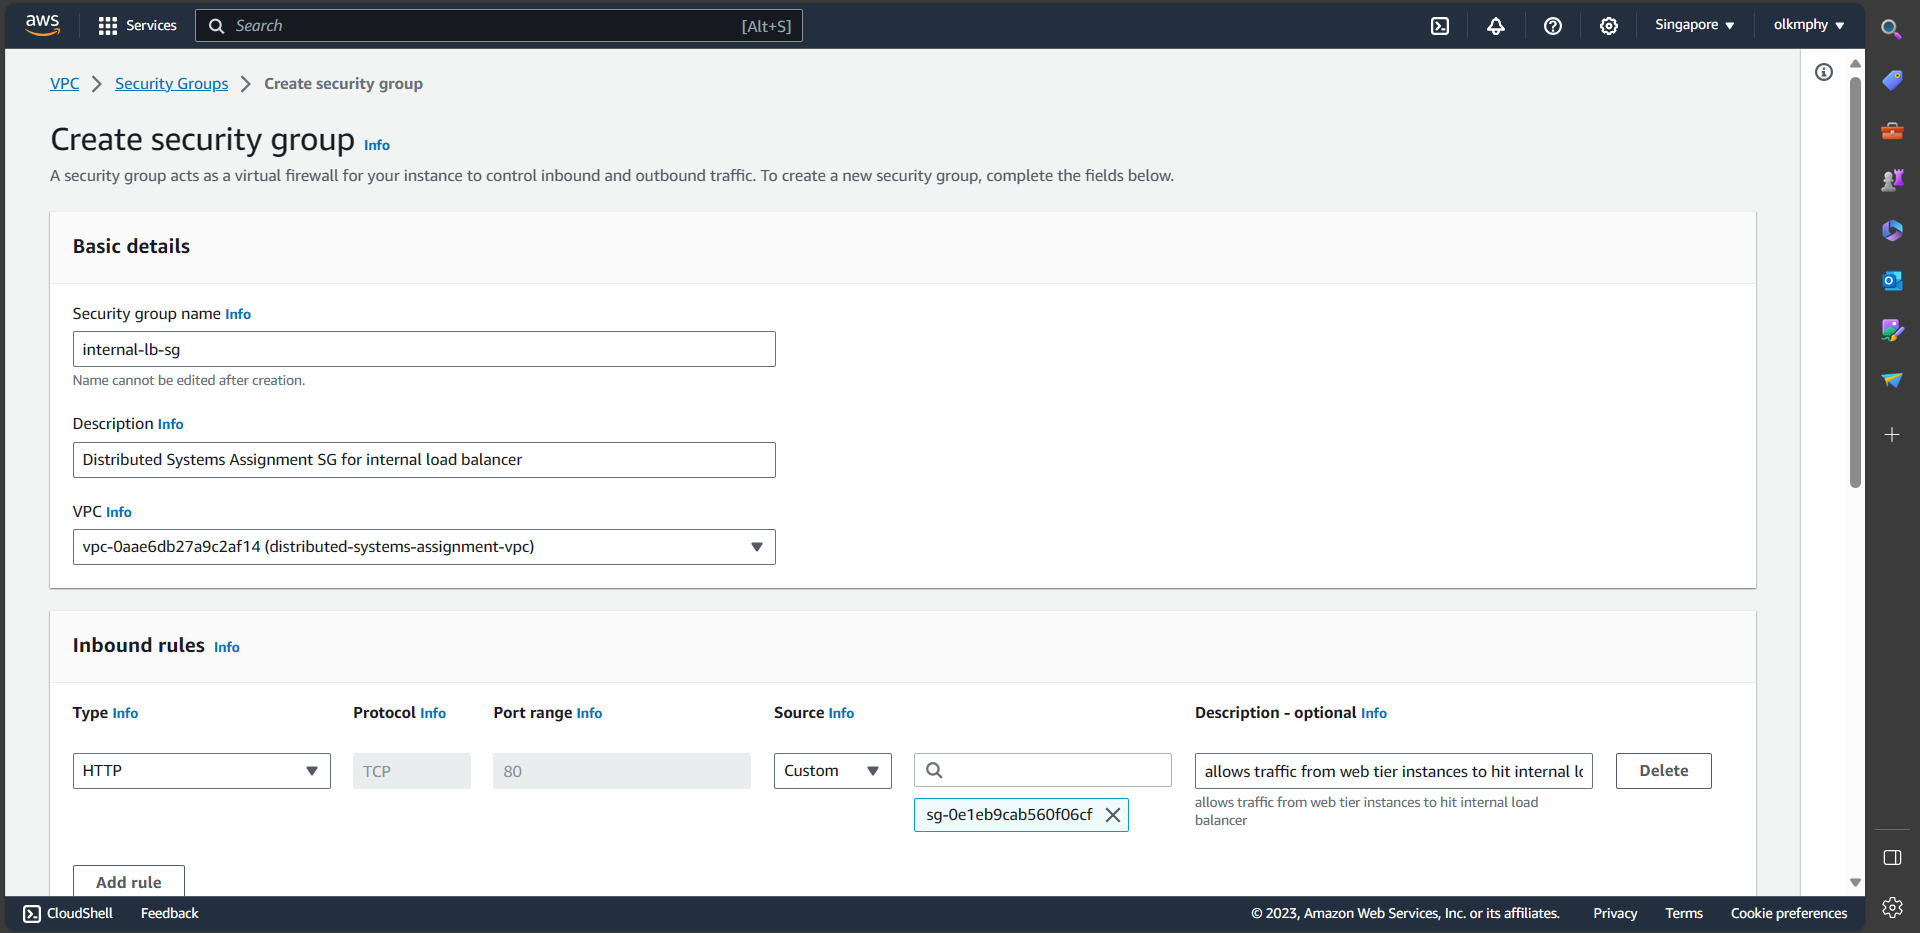
\includegraphics[width=12cm]{Pictures/Networking and Security/SG_create_3.png}
    \caption{Security Group for internal load balancer.}
    \label{fig:enter-label}
\end{figure}

We will set up the fourth security group dedicated to our private instances. Once provided a name and description, include an inbound rule permitting TCP traffic on port 4000 from the internal load balancer security group established earlier. This port corresponds to the application running on our app tier and enables the internal load balancer to direct traffic to our private instances. Additionally, I incorporate a rule for port 4000 allowing your IP for testing purposes.\par

\newpage
\begin{figure}[h]
    \centering
    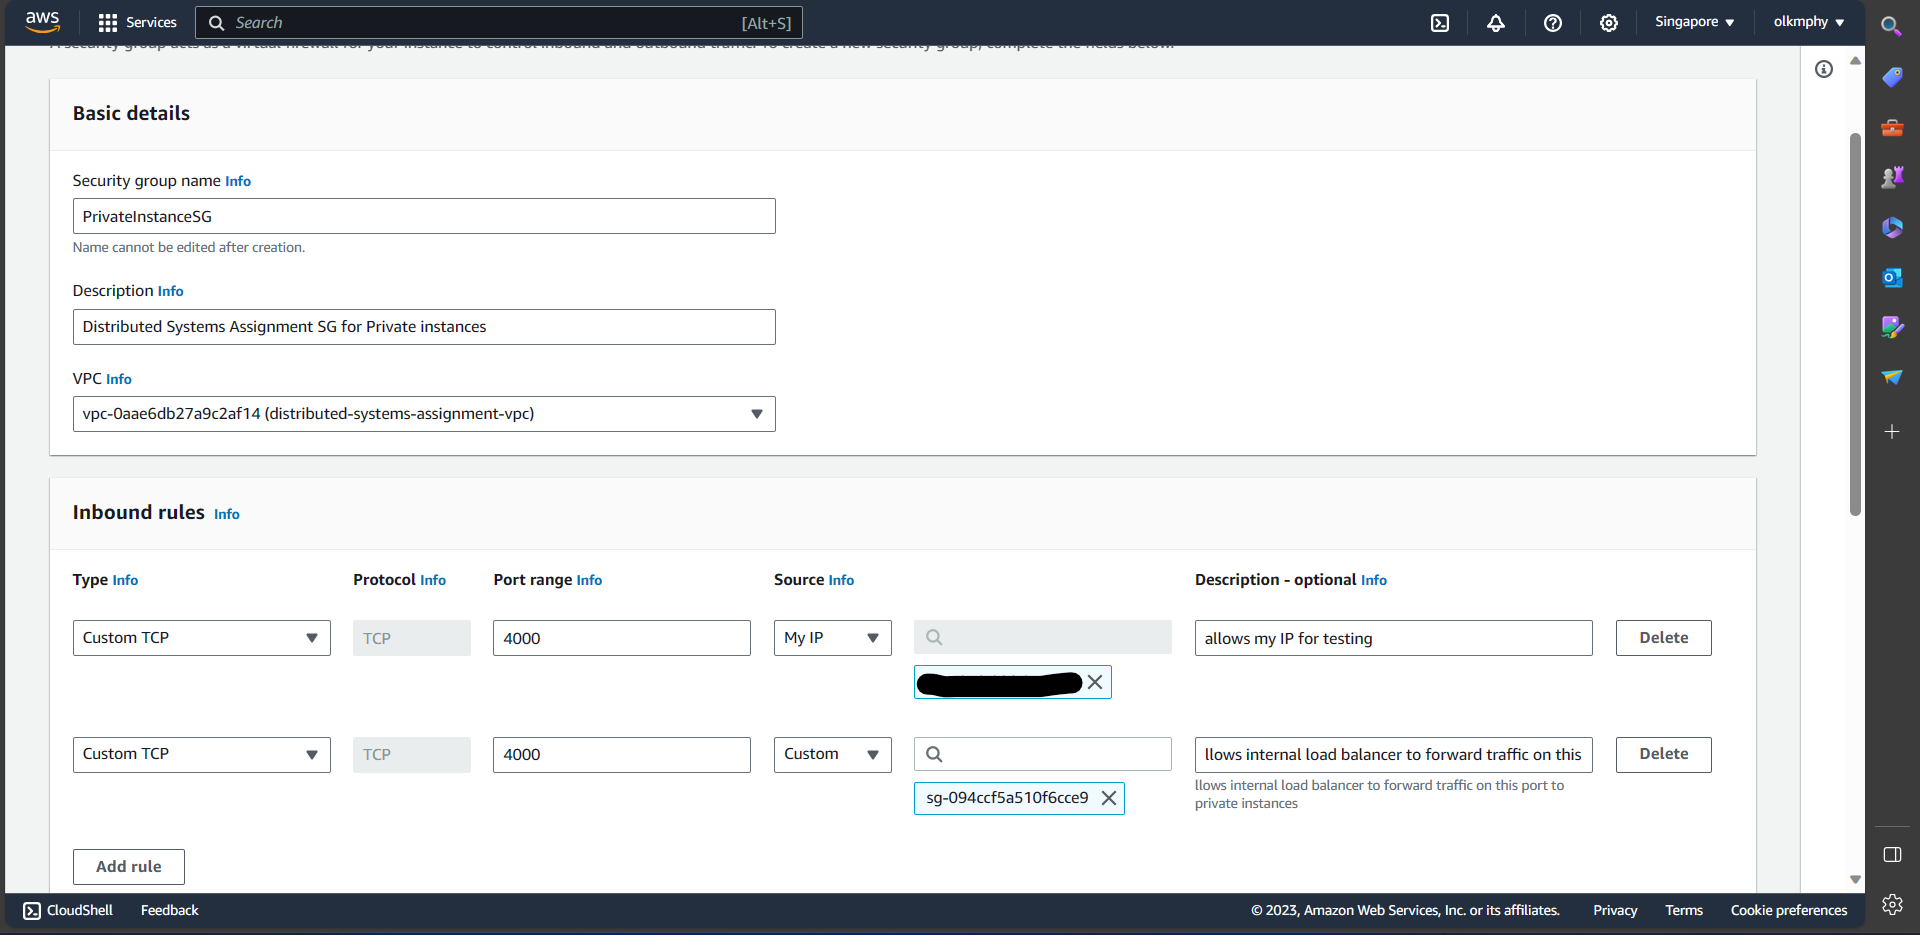
\includegraphics[width=12cm]{Pictures/Networking and Security/SG_create_4.png}
    \caption{Security group for the app-tier instance.}
    \label{fig:enter-label}
\end{figure}

The last security group that we will create is the security group for the Database-tier. For this security group, I add an inbound rule that will allow traffic from the private instance security group to the MYSQL/Aurora port (3306).

\begin{figure}[h]
    \centering
    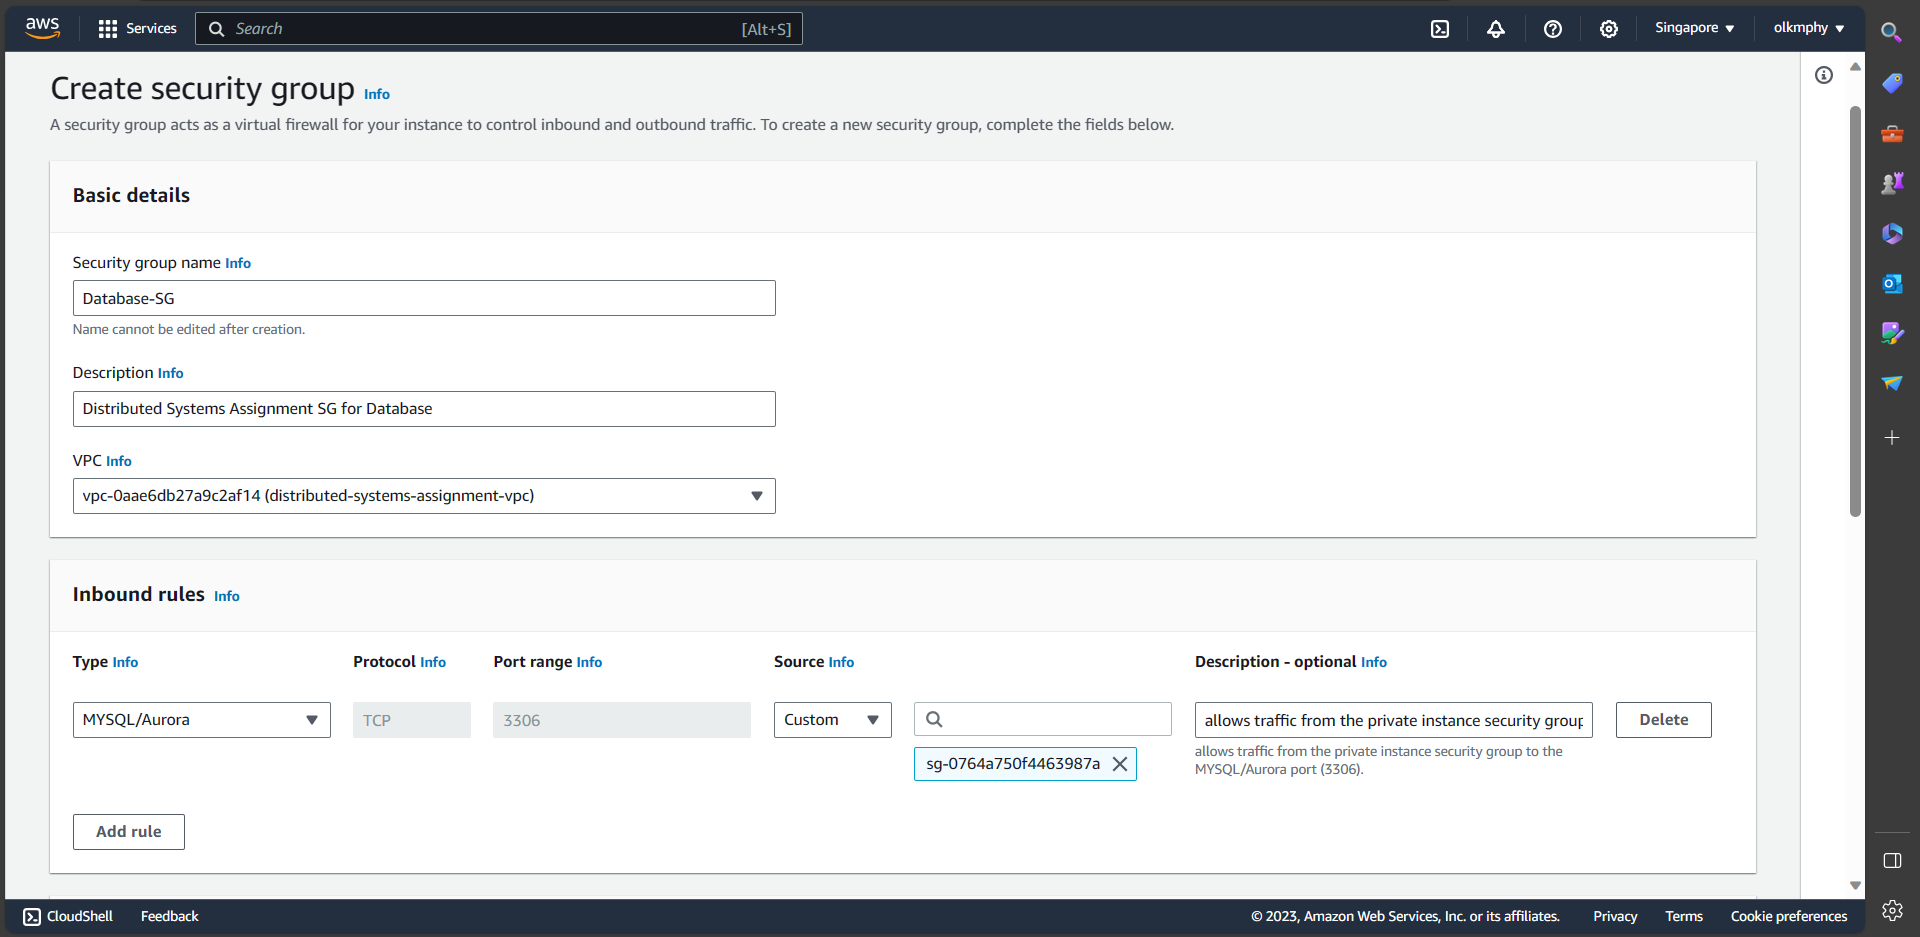
\includegraphics[width=12cm]{Pictures/Networking and Security/SG_create_5.png}
    \caption{Security group for database.}
    \label{fig:enter-label}
\end{figure}

After all, we have finished configuring the network and security for our application. Next step, we will start working with the database. I chose MySQL for this project and AWS supports a service called Amazon RDS to deploy my own database on a cloud platform. Using MySQL-Compatible Amazon Aurora.
\newpage

\subsection{Database}
First of all, I will create a Subnet Group. In Amazon RDS (Relational Database Service), a subnet group is used to define the set of subnets (specifically, Amazon Virtual Private Cloud (Amazon VPC) subnets) where your RDS DB instances will be created. It plays a crucial role in specifying the network configuration for the RDS DB instances.\par
In this Subnet Group, it will contain 2 private subnet for the database that I haved created early.\par
\begin{figure}[h]
    \centering
    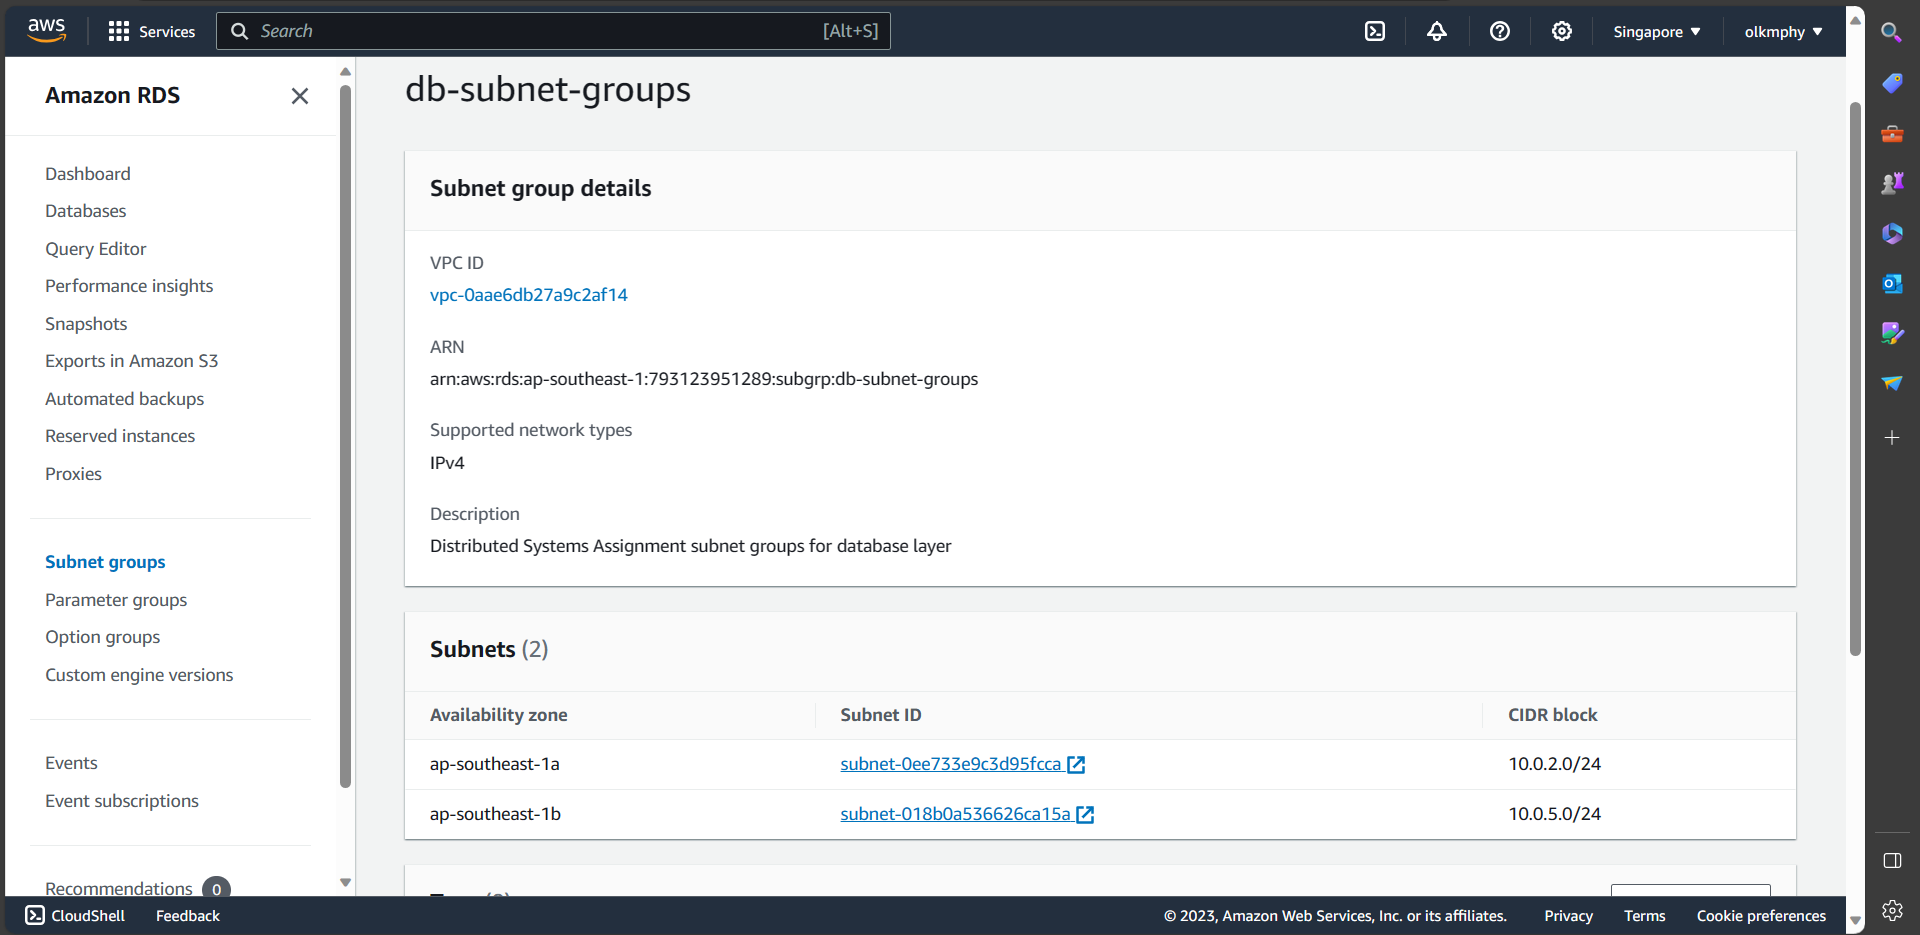
\includegraphics[width=12cm]{Pictures/Database/Subnet_group_create_1.png}
    \caption{Create Subnet Group in RDS.}
    \label{fig:enter-label}
\end{figure}

After creating the Subnet Group for the instances, I will then create the instances.\par 
\begin{figure}[h]
    \centering
    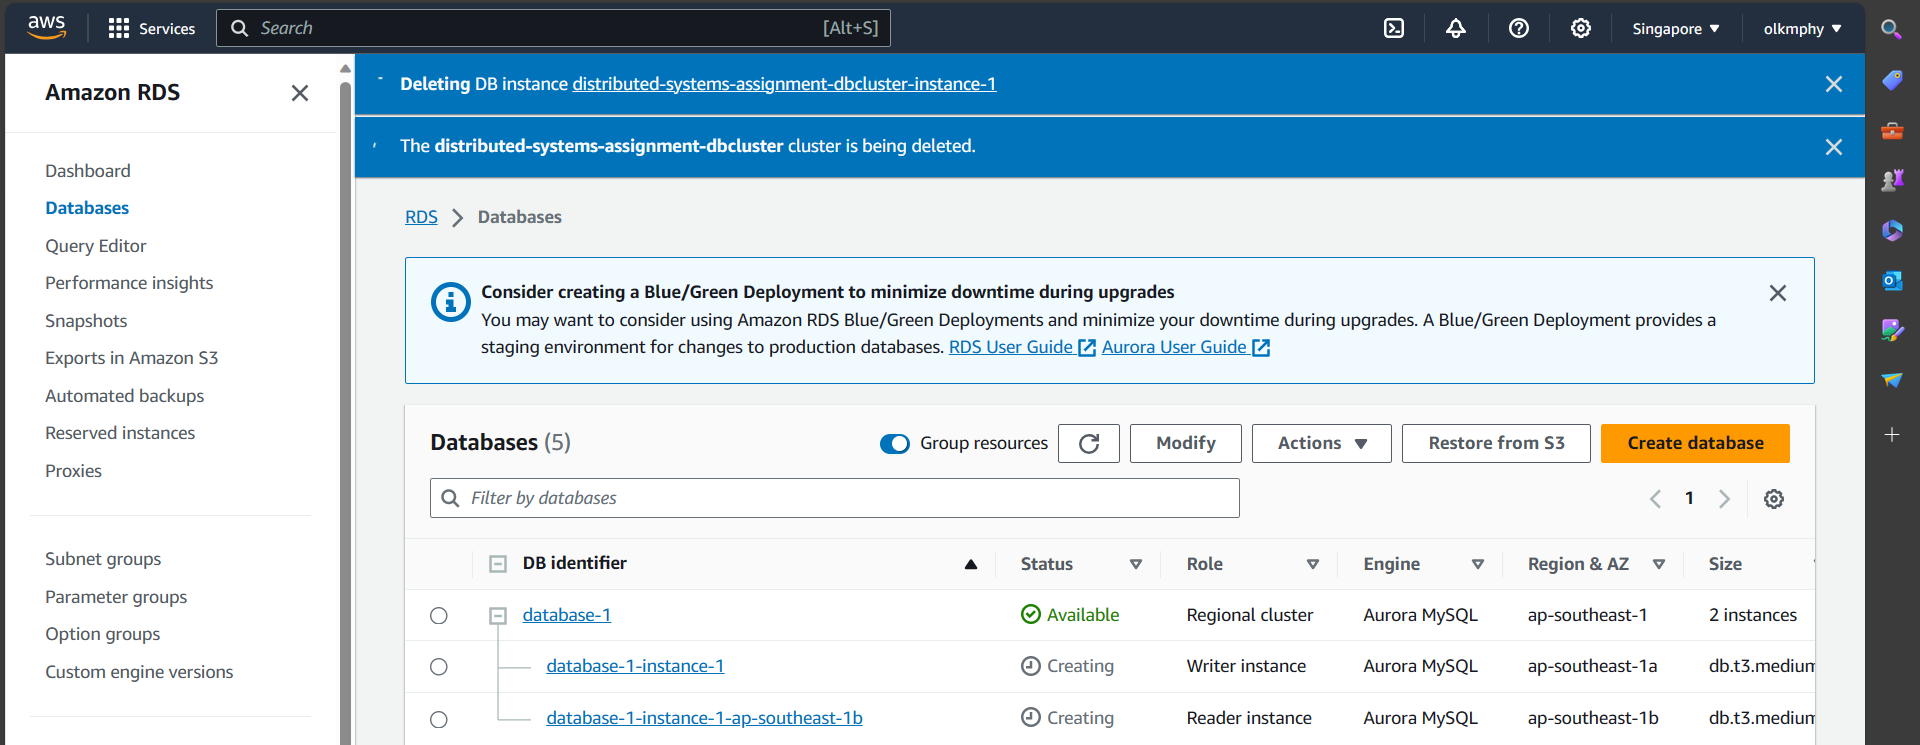
\includegraphics[width=12cm]{Pictures/Database/DB_create.png}
    \caption{Create MySQL database instances.}
    \label{fig:enter-label}
\end{figure}

Make sure that there will be two Aurora instances and each of them will be located in different subnets which belong to the Subnet Group that we have created before. One of them is \textbf{Writer instance} which is our main DB. We will process transactions using this DB. The other one is called \textbf{Reader instance} and this server is used to copy the content of the Writer for backup data in case the main server fail or something, etc.\par

After finishing creating the Aurora instances. Our next step is to implement the Application Tier.\par

\newpage
\subsection{Application Tier}
To begin with, we will first upload the application files into S3 bucket. Then, we will create our \textbf{AppLayer} instance. We will use the instance type of \textit{t2.micro} due to the free-tier availability. Here are the configurations of the instance before we create it.\par
\begin{figure}[h]
    \centering
    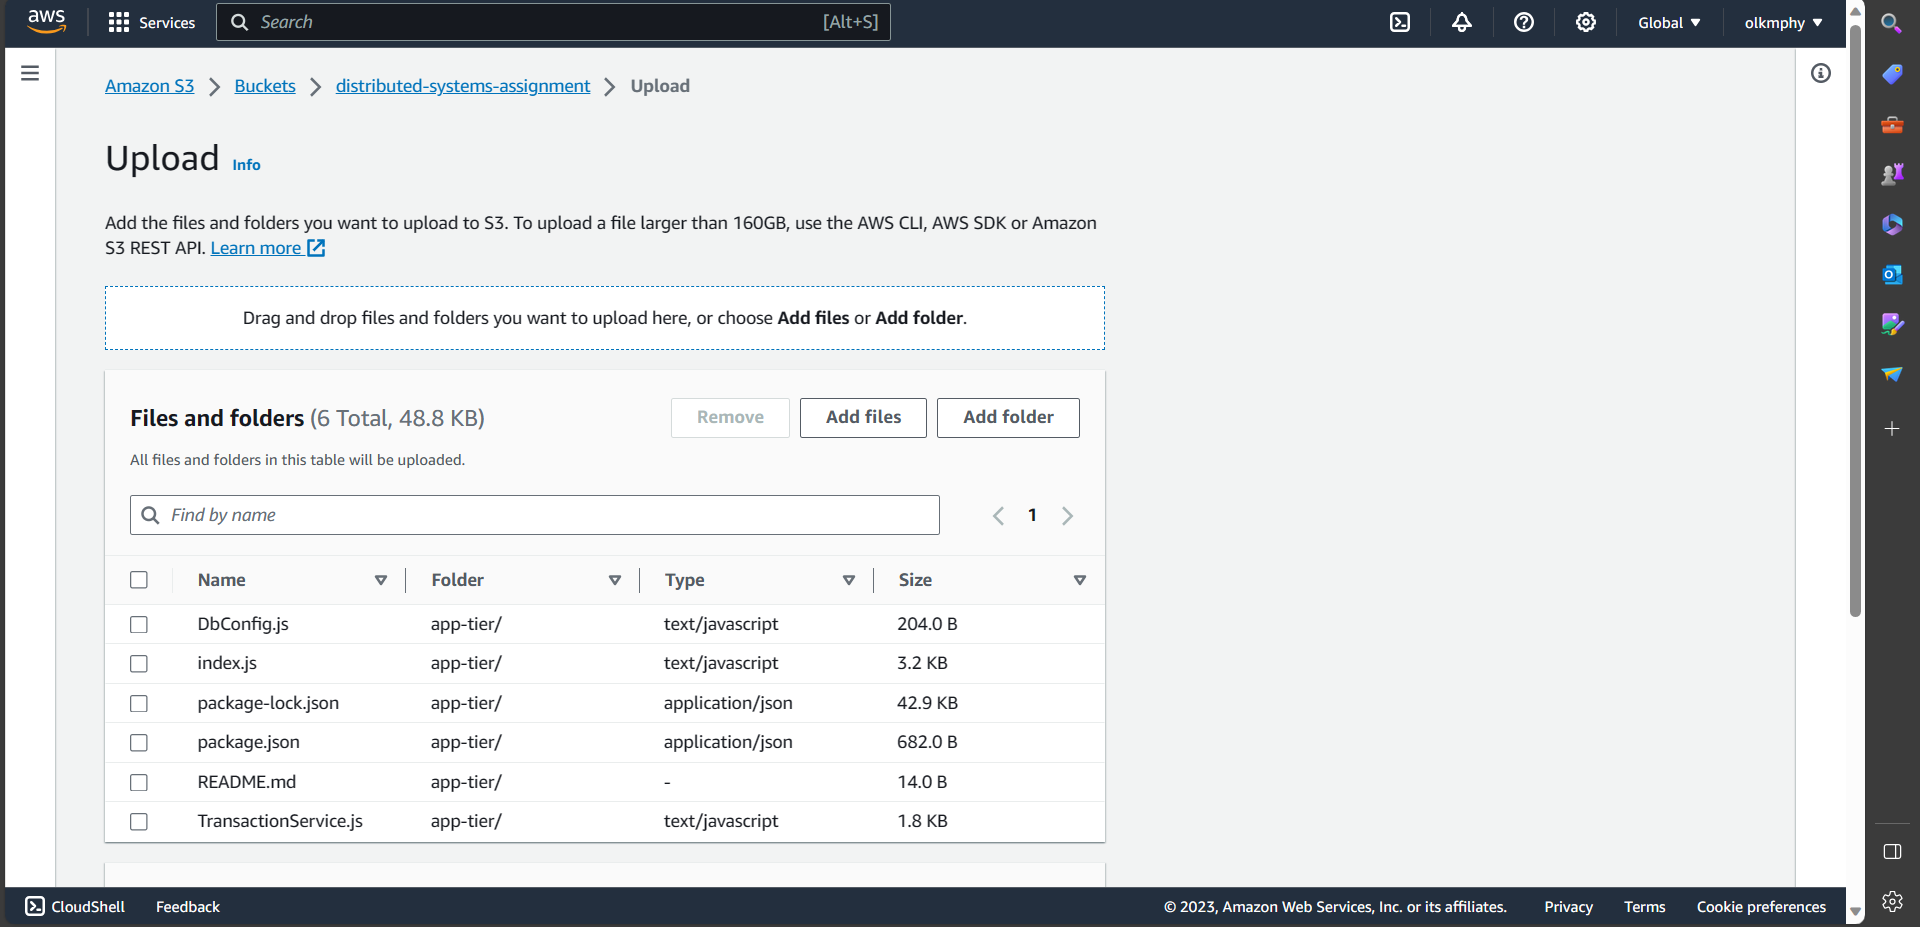
\includegraphics[width=12cm]{Pictures/App-tier/Upload_S3.png}
    \caption{Upload files to S3 bucket.}
    \label{fig:enter-label}
\end{figure}

\begin{figure}[h]
    \centering
    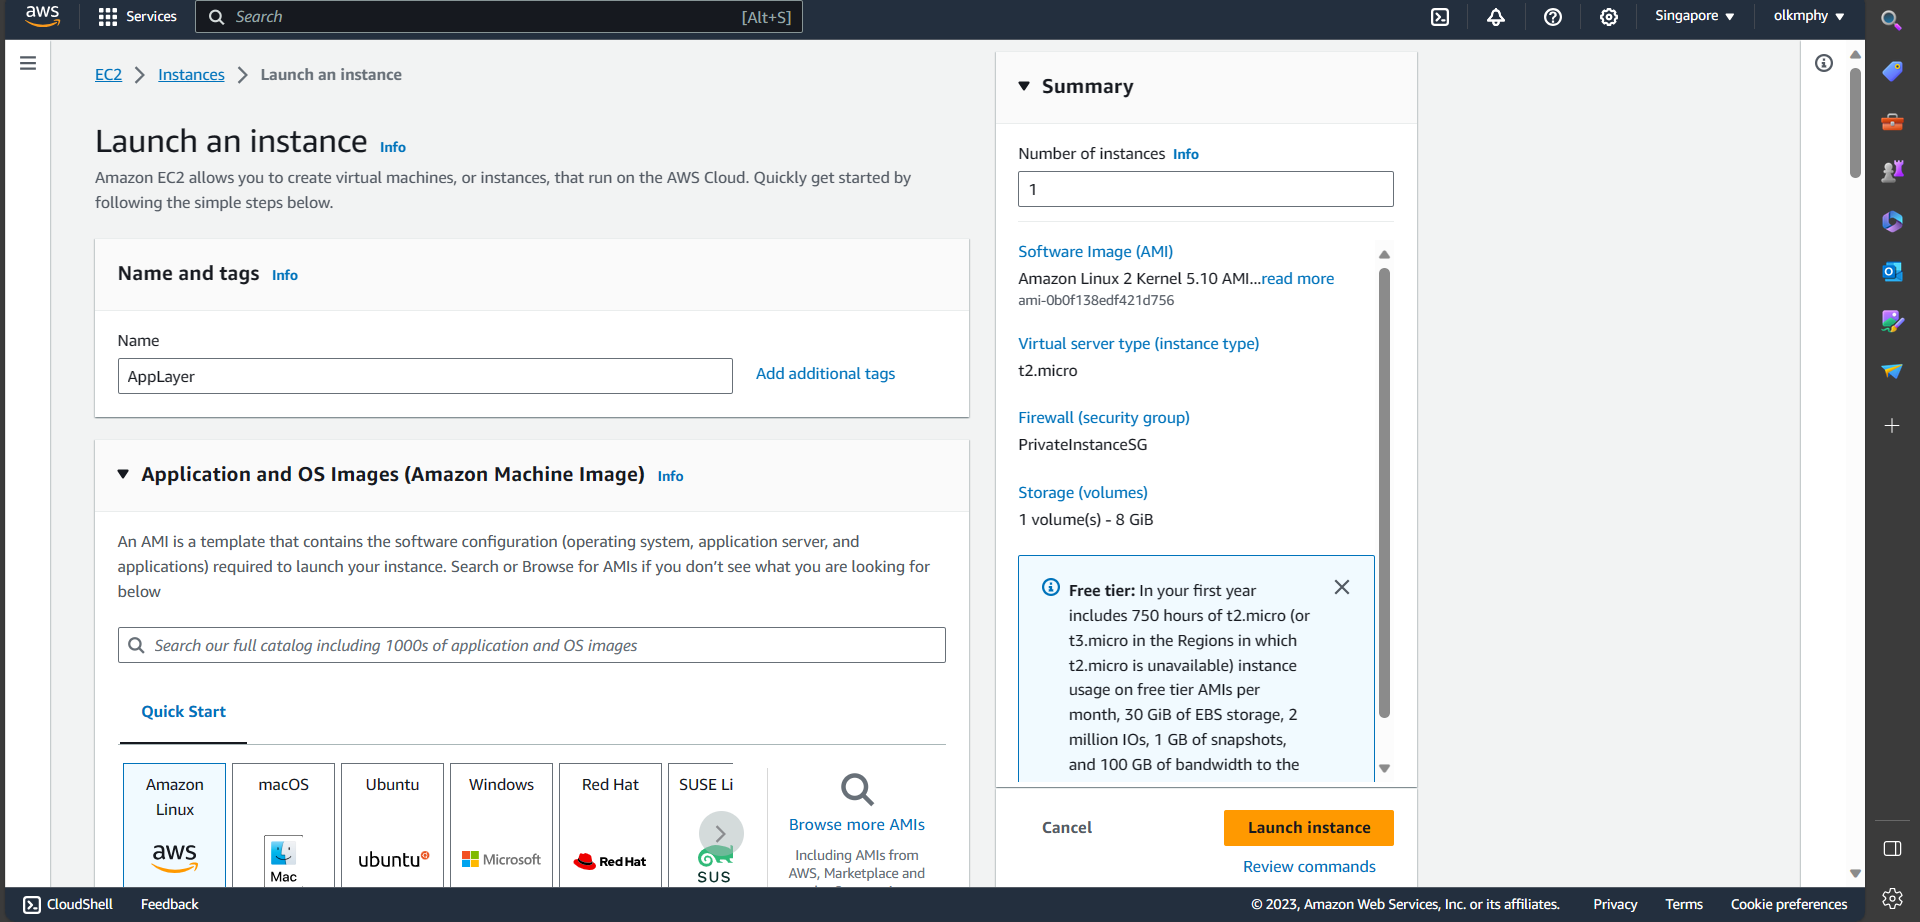
\includegraphics[width=12cm]{Pictures/App-tier/App_Instance_create.png}
    \caption{App Tier instance.}
    \label{fig:enter-label}
\end{figure}

After creating our \textbf{AppLayer} instance, we will connect to it and configure our deployment. First of all, we will have to connect the instance to the database that we have created before. Here are the bash command for it:\par

\begin{lstlisting}
sudo yum install mysql -y
\end{lstlisting}

By using this command, we will starting to download the MySQL CLI.\par

\begin{lstlisting}
mysql -h [RDS-ENDPOINT] -u admin -p
\end{lstlisting}
\begin{figure}[h]
    \centering
    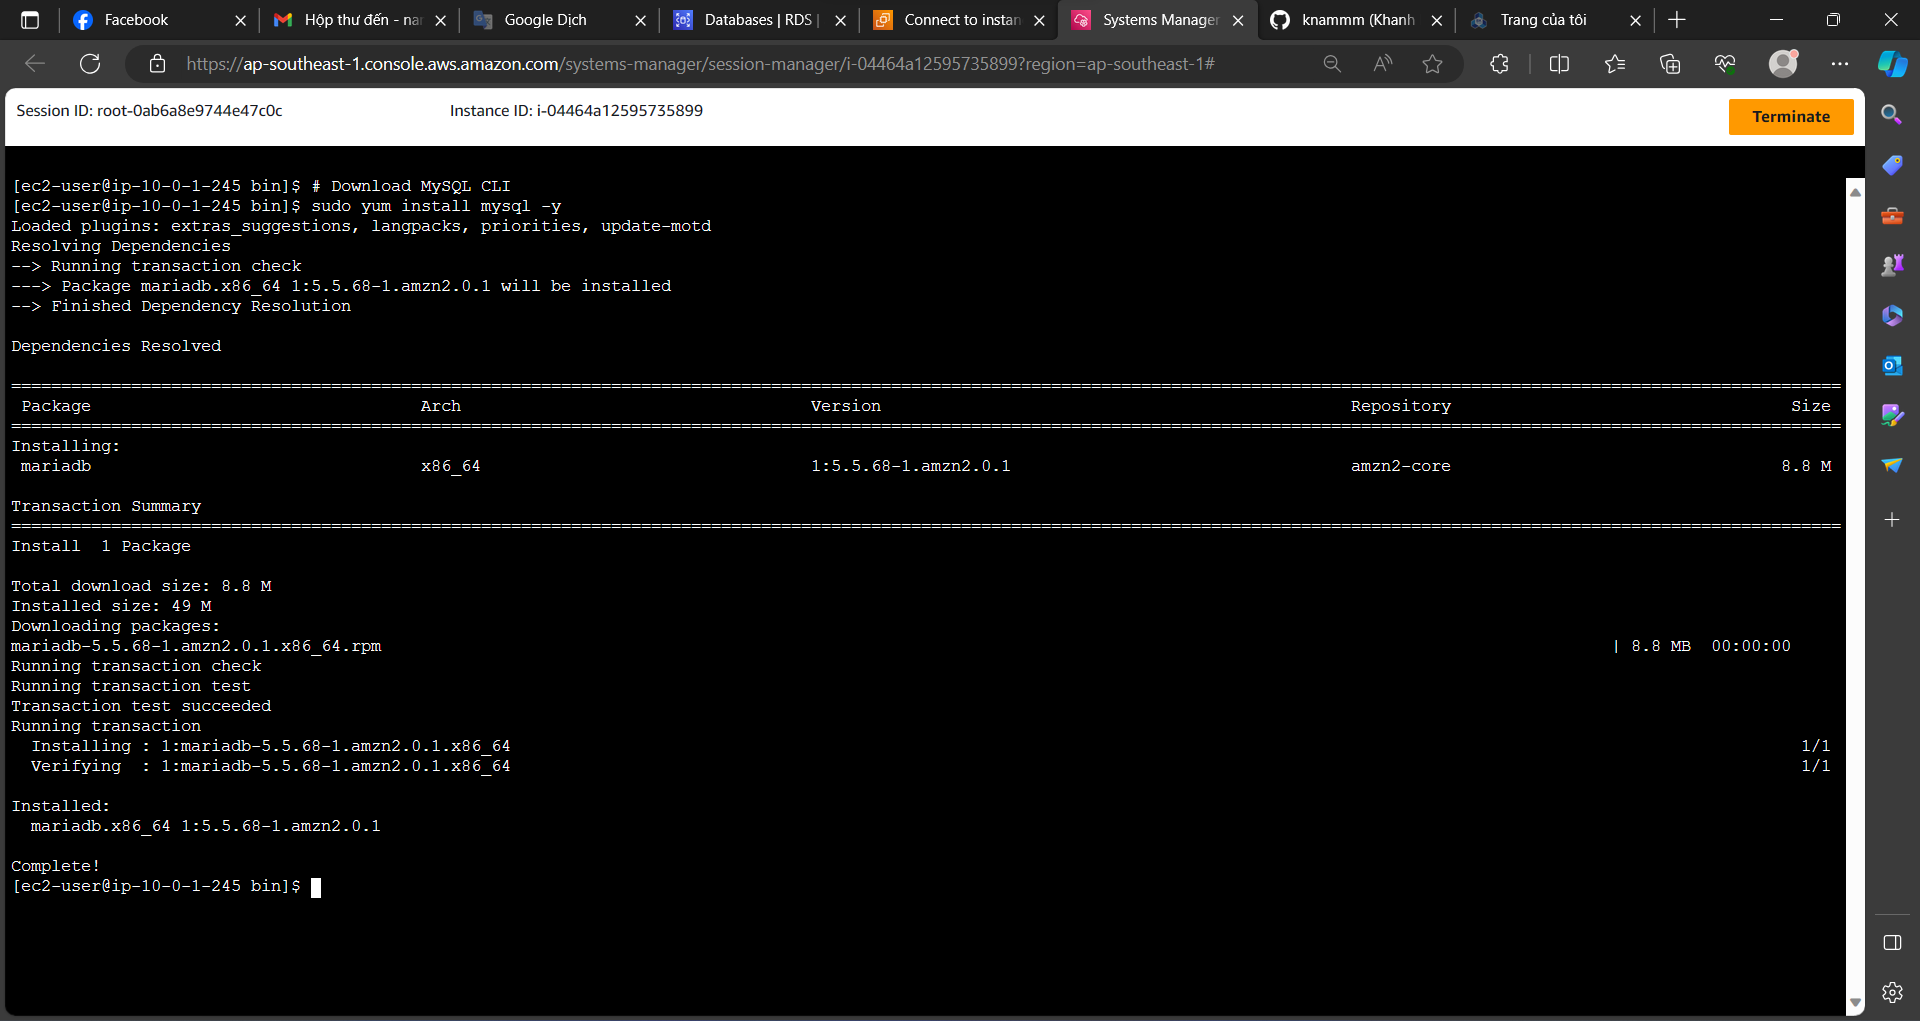
\includegraphics[width=12cm]{Pictures/App-tier/EC2_down_MySQL.png}
    \caption{Downloading MySQL CLI.}
    \label{fig:enter-label}
\end{figure}

\newpage
After that, we will connect to the database on the RDS that we have created before. Here is the result when we use the above command.\par
\begin{figure}[h]
    \centering
    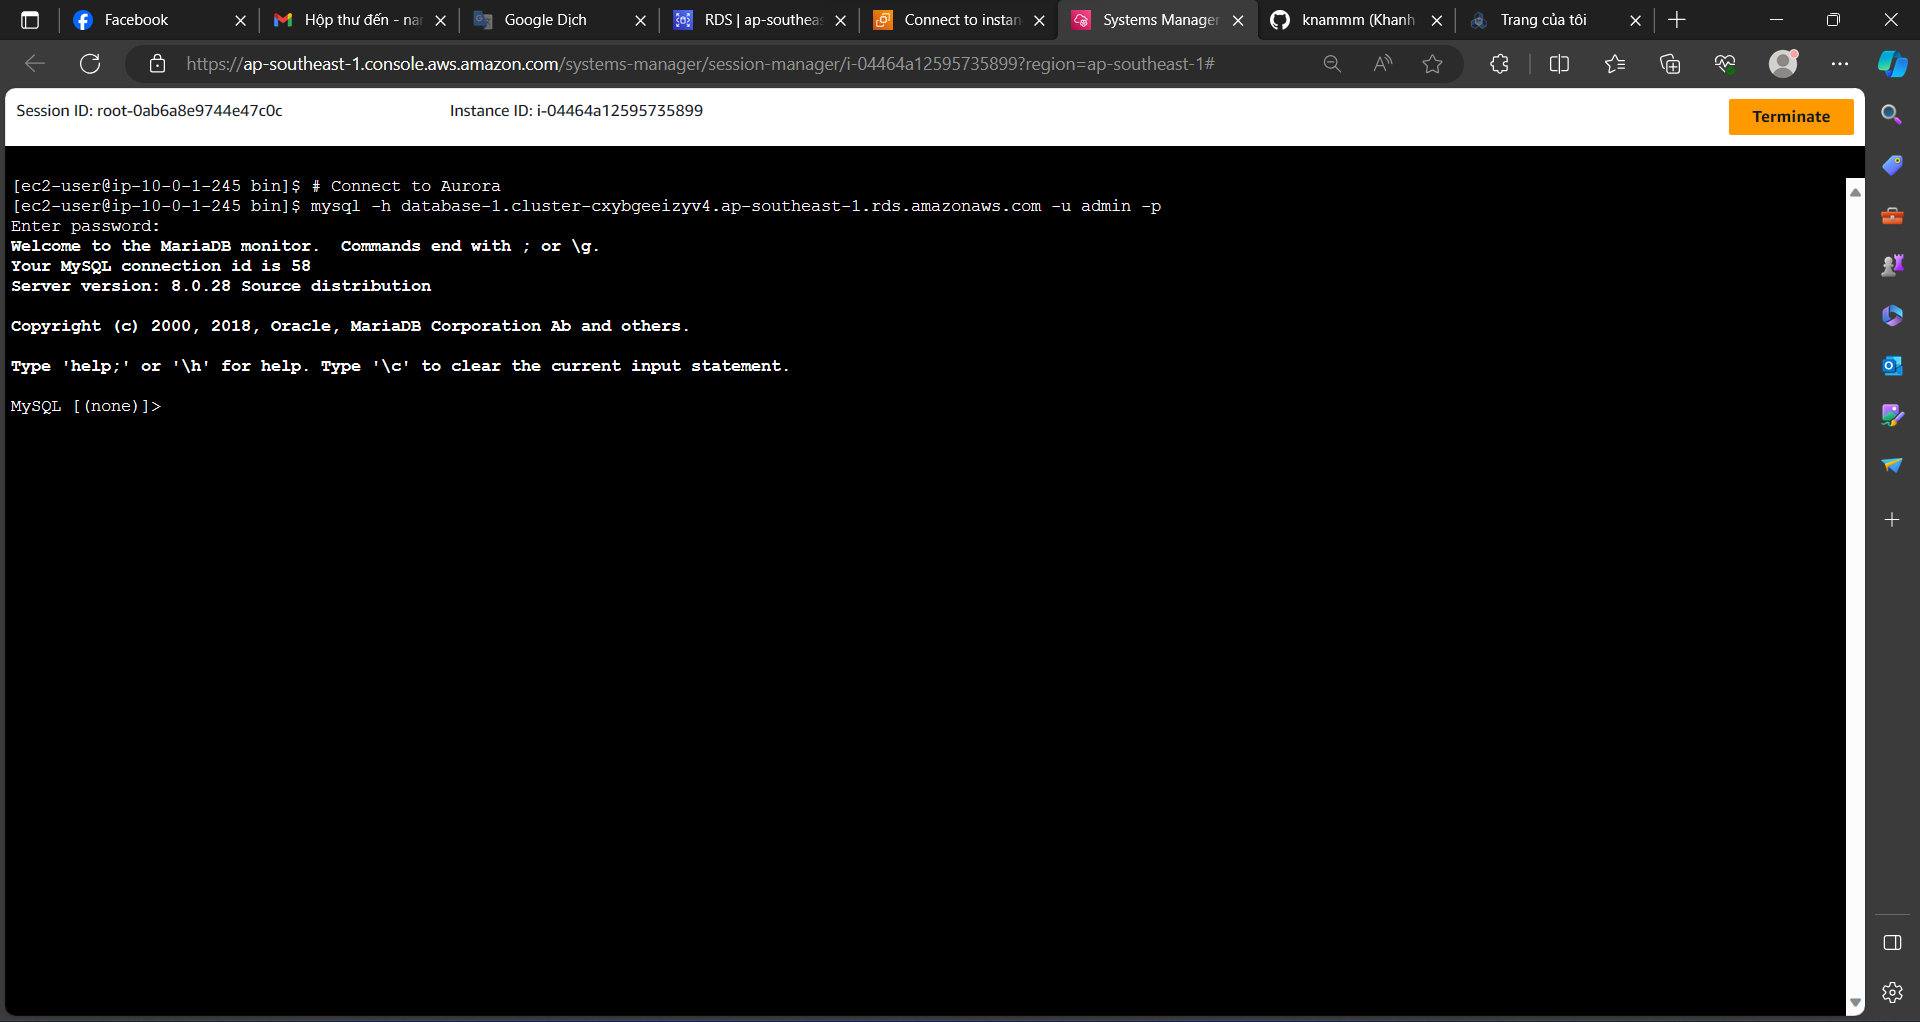
\includegraphics[width=12cm]{Pictures/App-tier/Connect_Aurora.png}
    \caption{Connect to Aurora database.}
    \label{fig:enter-label}
\end{figure}

Next, we will start to create a database called \textbf{webappdb} with the following command using the MySQL CLI:\par
\begin{lstlisting}
CREATE DATABASE webappdb;   
SHOW DATABASES;
USE webappdb;    
\end{lstlisting}

Then, we will create the following transactions table by executing this create table command and insert a test data into the table. Using these commands:\par
\begin{lstlisting}
CREATE TABLE IF NOT EXISTS transactions(id INT NOT NULL AUTO_INCREMENT, amount DECIMAL(10,2), description VARCHAR(100), PRIMARY KEY(id));
INSERT INTO transactions (amount,description) VALUES ('792003','KNAMMM');   
SELECT * FROM transactions;
\end{lstlisting}

Here is the output of the above commands:\par
\begin{figure}[h]
    \centering
    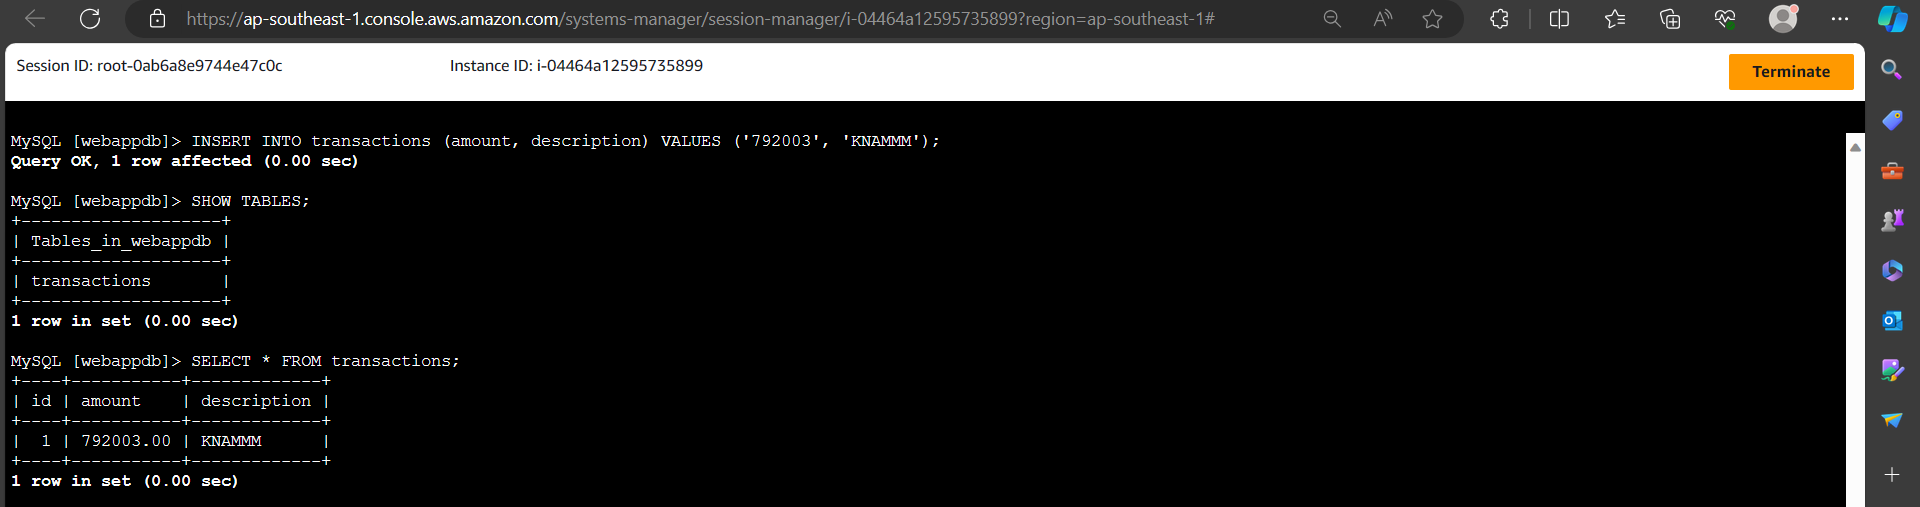
\includegraphics[width=12cm]{Pictures/App-tier/Insert_DB.png}
    \caption{Insert data into the table.}
    \label{fig:enter-label}
\end{figure}

\newpage
Now, I will configure our app instance. Downloading Node Version Manager (NVM) is the first step. Starting with these following commands:\par
\begin{lstlisting}
curl -o- https://raw.githubusercontent.com/nvm-sh/nvm/v0.38.0/install.sh | bash
source ~/.bashrc
\end{lstlisting}

Next, choose a compatible version of Node.js and download it to our App-Tier instance.\par
\begin{lstlisting}
nvm install 16
nvm use 16
\end{lstlisting}

\begin{figure}[h]
    \centering
    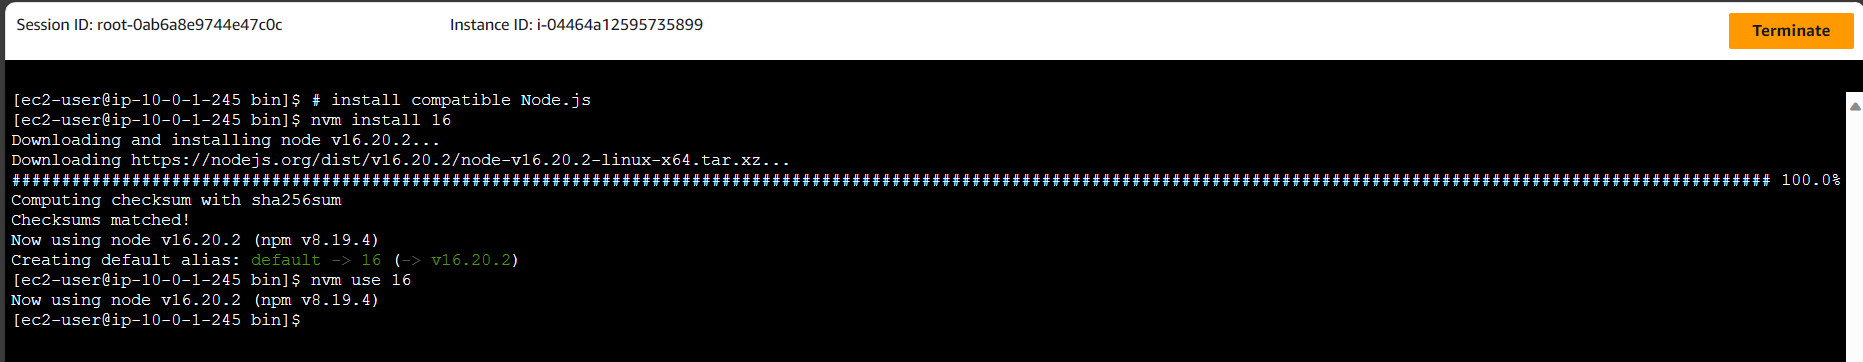
\includegraphics[width=12cm]{Pictures/App-tier/install nodejs.png}
    \caption{Install Node.js}
    \label{fig:enter-label}
\end{figure}

PM2 is a process manager for Node.js applications. It ensures the continuous operation of your Node.js app by keeping it running even if the hosting instance is exited or experiences a reboot. PM2 provides features like automatic restarts, logging, and monitoring, making it a valuable tool for maintaining the availability and stability of Node.js applications in production environments.\par

\begin{figure}[h]
    \centering
    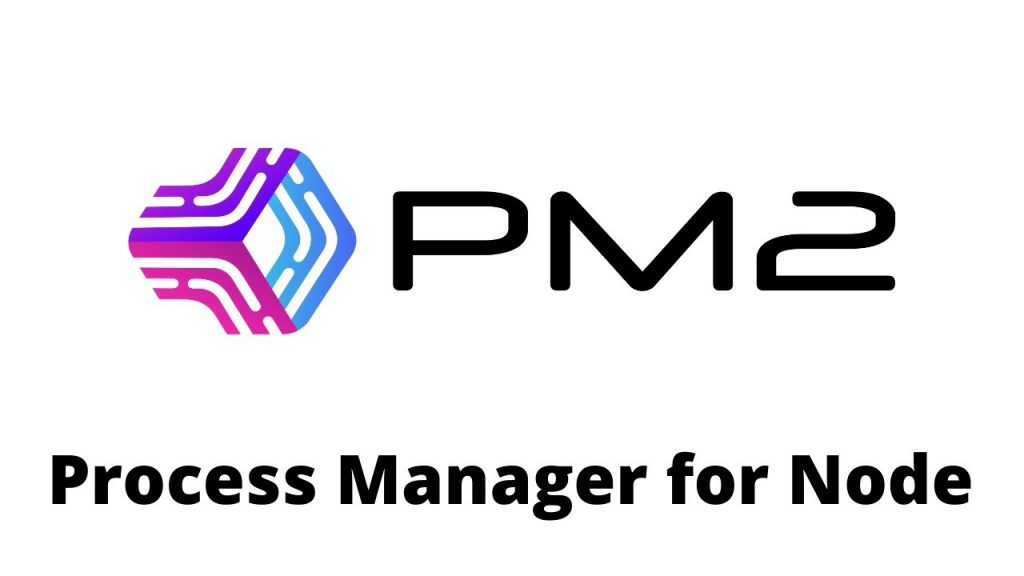
\includegraphics[width=12cm]{Pictures/App-tier/PM2.jpg}
    \caption{Process Manager for Node}
    \label{fig:enter-label}
\end{figure}

Using this command to install pm2:\par
\begin{lstlisting}
npm install -g pm2
\end{lstlisting}

\begin{figure}[h]
    \centering
    \includegraphics{Pictures/App-tier/install pm2.png}
    \caption{Installing pm2.}
    \label{fig:enter-label}
\end{figure}

\newpage
Now we need to download our code from our s3 buckets onto our instance. In the command below, replace \textit{BUCKET\_NAME} with the name of the bucket uploaded the app-tier folder to.\par
\begin{lstlisting}
aws s3 cp s3://[BUCKET_NAME]/app-tier/ app-tier --recursive
\end{lstlisting}

Now, navigate to the app-tier directory, install dependencies, and start the app with pm2. Using the following commands:\par
\begin{lstlisting}
cd ~/app-tier
npm install
pm2 start index.js
\end{lstlisting}

\begin{figure}[h]
    \centering
    \includegraphics[width=12cm]{Pictures/App-tier/run_app.png}
    \caption{Run back-end application.}
    \label{fig:enter-label}
\end{figure}

To check if pm2 is working correctly, we will use the commands:\par
\begin{lstlisting}
pm2 list
pm2 logs
\end{lstlisting}

\begin{figure}[h]
    \centering
    \includegraphics[width=12cm]{Pictures/App-tier/Check_active.png}
    \caption{Check pm2.}
    \label{fig:enter-label}
\end{figure}

\newpage
Make sure app stays running when user leaving the SSM session:\par

\begin{lstlisting}
pm2 startup
sudo env PATH=$PATH:/home/ec2-user/.nvm/versions/node/v16.0.0/bin /home/ec2-user/.nvm/versions/node/v16.0.0/lib/node_modules/pm2/bin/pm2 startup systemd -u ec2-user —hp /home/ec2-user
pm2 save
\end{lstlisting}

The last step, we will check if our app is running correctly or not:\par
\begin{lstlisting}
curl http://localhost:4000/health
curl http://localhost:4000/transaction
\end{lstlisting}

\begin{figure}[h]
    \centering
    \includegraphics[width=12cm]{Pictures/App-tier/Check_health&DB.png}
    \caption{Check health and DB connectivity.}
    \label{fig:enter-label}
\end{figure}

After we have finished configuringthe app-tier instance, we will then create the internal load balancer and scale servers so that the load balancer will distribute the connectivity.\par
\newpage

\subsection{Internal Load Balancer and Auto Scaling Group}
First of all, we will create the image of the app-tier server that we have configured so far in the above section. This image will entail all the information of the previous server's configuration so that we can scale multiple servers based on that layout.\par

Next step, we are going to create a Target Group. The purpose of forming this target group is to use with our load blancer so it may balance traffic across our private app tier instances.\par

\begin{figure}[h]
    \centering
    \includegraphics[width=12cm]{Pictures/Internal LB/TG_create.png}
    \caption{Create target group in private subnets.}
    \label{fig:enter-label}
\end{figure}

After establishing the target group, the next step is to set up an internal load balancer that directs traffic to the instances.\par

\begin{figure}[h]
    \centering
    \includegraphics[width=12cm]{Pictures/Internal LB/internal_lb_4.png}
    \caption{Internal Load Balancer creation.}
    \label{fig:enter-label}
\end{figure}

Before we configure Auto Scaling, we need to create a Launch template with the AMI we created earlier.\par

Finally is to create the Auto Scaling Group for our AppLayer so that we can scale many instances as we desire. Following the steps:\par
\newpage
\begin{figure}[h]
    \centering
    \includegraphics[width=12cm]{Pictures/Internal LB/ASG_1.png}
    \caption{Step 1.}
    \label{fig:enter-label}
\end{figure}
Step one is to choose the template of the app instance that we have created before so that the ASG can create new instances with the configurations entailed from the template.\par

\begin{figure}[h]
    \centering
    \includegraphics[width=12cm]{Pictures/Internal LB/ASG_2.png}
    \caption{Step 2.}
    \label{fig:enter-label}
\end{figure}

The second step is to choose the private subnets so that the instances will be created in those subnets.\par

\begin{figure}[h]
    \centering
    \includegraphics[width=12cm]{Pictures/Internal LB/ASG_3.png}
    \caption{Step 3.}
    \label{fig:enter-label}
\end{figure}

Third step is to attached the ASG with the internal load balancer that we have created before so that the internal-lb can distribute traffic to the instances.\par
\newpage

Step four is to choose the group size which means that the desired number of instances. In this assignment, I will choose two.
\begin{figure}[h]
    \centering
    \includegraphics[width=12cm]{Pictures/Internal LB/ASG_4.png}
    \caption{Step 4.}
    \label{fig:enter-label}
\end{figure}

After all, it can be seen that there will be two new instances that have been created after we have finished configured our Auto Scaling Group. And to sum up, these new instances will have the same configurations with the previous AppLayer instance before.\par
\begin{figure}[h]
    \centering
    \includegraphics[width=12cm]{Pictures/Internal LB/ASG_5.png}
    \caption{Two new App-Instance have been created.}
    \label{fig:enter-label}
\end{figure}

\newpage

\subsection{Web Tier}
Before we create and configure the web instances, we will first replace the [INTERNAL-LOADBALANCER-DNS] in the nginx.conf file. And then upload both web-tier folder and nginx.conf files to the S3 bucket.\par
\begin{figure}[h]
    \centering
    \includegraphics[width=12cm]{Pictures/Web-tier/nginx conf.png}
    \caption{Replace Internal LB DNS.}
    \label{fig:enter-label}
\end{figure}

Next, I will create the web-instance.\par
\begin{figure}[h]
    \centering
    \includegraphics[width=12cm]{Pictures/Web-tier/EC2_create.png}
    \caption{EC2 instance create.}
    \label{fig:enter-label}
\end{figure}

When the server is ready, the next step is to configure the web-tier server. Start by connecting to the server through SSM. Using the following bash commands:\par

\begin{lstlisting}
sudo -su ec2-user
curl -o- https://raw.githubusercontent.com/nvm-sh/nvm/v0.38.0/install.sh | bash
source ~/.bashrc
nvm install 16
nvm use 16
\end{lstlisting}

Followed by downloading the source code of web-tier from S3 bucket to our instance. Using the commands:\par
\begin{lstlisting}
cd ~/
aws s3 cp s3://[BUCKET_NAME]/web-tier/ web-tier --recursive
\end{lstlisting}

Subsequently, go to the web-layer directory and establish the build folder for the React app to facilitate serving our code:\par
\begin{lstlisting}
cd ~/web-tier
npm install 
npm run build
\end{lstlisting}

\begin{figure}[h]
    \centering
    \includegraphics[width=12cm]{Pictures/Web-tier/npm_build.png}
    \caption{Build folder for the React App.}
    \label{fig:enter-label}
\end{figure}

NGINX has various applications such as load balancing and content caching. However, in our case, we will utilize it as a web server configured to host our application on port 80. Additionally, it will assist in directing our API calls to the internal load balancer.\par

\begin{lstlisting}
sudo amazon-linux-extras install nginx1 -y
cd /etc/nginx
ls
\end{lstlisting}

We should see an nginx.conf file here. We’re going to delete this file and use the one we uploaded to S3.\par
\begin{lstlisting}
sudo rm nginx.conf
sudo aws s3 cp s3://[BUCKET_NAME]/nginx.conf .
\end{lstlisting}

Afterward, restart Nginx. Ensure that Nginx has the necessary permissions to access our files, and verify that the service initiates on system boot by executing these commands:\par
\begin{lstlisting}
sudo service nginx restart
chmod -R 755 /home/ec2-user
sudo chkconfig nginx on
\end{lstlisting}

After this step, when I input the public IP address of the web tier instance, I'll be able to access the website. The database is properly connected and functioning, I can also observe its functionality. In addition, inserting data into the database or delete data in the database, etc.\par

\begin{figure}[h]
    \centering
    \includegraphics[width=12cm]{Pictures/Internet/Result_1.png}
    \caption{Home page of the App.}
    \label{fig:enter-label}
\end{figure}

After finishing configuring the web-tier instance. We will then continue to deploy the External(Internet-facing) Load Balancer and Auto Scaling Group for the WebTier. The steps is almost the same as \textbf{Internal Load Balancer and Auto Scaling Group} instead of changing the load balancer from internal into internet-facing.\par

\subsection{Result}
After all, here are the results of the application.\par

\begin{figure}[h]
    \centering
    \includegraphics[width=12cm]{Pictures/Internet/Result_1.png}
    \caption{Home page of the App.}
    \label{fig:enter-label}
\end{figure}

\begin{figure}[h]
    \centering
    \includegraphics[width=12cm]{Pictures/Internet/Result_2.png}
    \caption{Demo Database.}
    \label{fig:enter-label}
\end{figure}
\newpage

Now I will test some database functions. Starting by \textbf{adding} some new elements.\par
\begin{figure}[h]
    \centering
    \includegraphics[width=12cm]{Pictures/Internet/Result_3.png}
    \caption{Add new elements.}
    \label{fig:enter-label}
\end{figure}

Next, let's test the \textbf{deletion by ID}.\par
\begin{figure}[h]
    \centering
    \includegraphics[width=10cm]{Pictures/Internet/Delete_1.png}
    \caption{Delete by ID interface.}
    \label{fig:enter-label}
\end{figure}

\begin{figure}[!htp]
    \centering
    \includegraphics[width=10cm]{Pictures/Internet/Delete_2.png}
    \caption{Element deleted.}
    \label{fig:enter-label}
\end{figure}
\newpage
Also test the \textbf{deleteAll} function.\par
\begin{figure}[h]
    \centering
    \includegraphics[width=12cm]{Pictures/Internet/DeleteAll_1.png}
    \caption{Delete All interface.}
    \label{fig:enter-label}
\end{figure}

\begin{figure}[h]
    \centering
    \includegraphics[width=12cm]{Pictures/Internet/DeleteAll_2.png}
    \caption{All the elements have been deleted.}
    \label{fig:enter-label}
\end{figure}
\newpage

Finally, checking the back-end instances log:\par
\begin{figure}[h]
    \centering
    \includegraphics[width=12cm]{Pictures/Internet/AppIns_1.png}
    \caption{AppLayer Instance 1st.}
    \label{fig:enter-label}
\end{figure}

\begin{figure}[h]
    \centering
    \includegraphics[width=12cm]{Pictures/Internet/AppIns_2.png}
    \caption{AppLayer Instance 2nd.}
    \label{fig:enter-label}
\end{figure}

It's evident that the internal load balancer effectively routes information to the instances. We observe a distribution of transactions across multiple instances, rather than a single instance handling all transactions. Transactions are randomly distributed to any of the instances within the AppLayer.

\newpage
\section{Summary}
After completing the mini project "Deploying a 3-tier web application using AWS," I have learned many important things and had valuable experiences. Here are the key lessons that I have learned from this project:\par

\textbf{Understanding basic concepts of AWS:} The project helped me develop a solid architecture of AWS services, especially EC2, RDS, and S3. I master declarative development, management, and integration to build high-performance applications.\par

\textbf{Knowledge of 3-Tier Architecture:} Learn how to build a 3-tier architecture with Presentation Layer, Application Layer, and Database Layer. I applied these principles to create a system that is structured, easy to maintain, and scalable.\par

\textbf{Managing Resources in Amazon VPC:} Learn how to use Amazon VPC to create a virtual installation environment for my resources. I understand how to manage subnets, routing tables, and security groups to ensure security and availability.\par

\textbf{Using Amazon RDS for Database Management:} Learn about Amazon RDS and how it enables effective database management. This tuning includes simple database creation, backup, and restore.\par

\textbf{Managing Resources in AWS S3:} Learn how to use Amazon S3 to store and manage application's static resources. Understood how to configure groups, access permissions, and integrate it into the application.\par

\textbf{Security Problem:} Apply security measures such as IAM Roles and Security Groups to ensure application and data security.\par

\textbf{Dynamic Load Balancing:} Understand how to implement dynamic load balancing to distribute work efficiently among instances. This feature helps optimize resources and ensures easy scalability with additional load.\par

\textbf{Error Handling and Recovery:} Develop error handling and recovery strategies to ensure that the system is fault tolerant and able to recover quickly when problems occur.\par

\textbf{Session and Health Management:} Learn how to manage user sessions and health in distributed environments. This involves maintaining session state between requests and layers of the system.\par

Since I was still taking advantage of the free plan, I faced specific limitations related to the configuration of the instances. However, in AWS, you have a wide range of server options available with powerful configurations, but this often comes at a high cost. This corresponds to the "pay-as-you-go" philosophy of the cloud service model.\par

In total, the project helped me step by step to become an automated AWS developer, capable of developing and managing complex web applications in a cloud environment. This lesson not only provides theoretical knowledge but also provides important practical experience in building high-performance and reliable systems.\par

\vspace{10pt}
If you have any problem, please contact via email: \url{nam.nguyenolkmphy@hcmut.edu.vn}\par
The source code of the project will be available here: \href{https://github.com/knammm/Three-Tier-Web-Application}{GitHub}


\newpage

\bibliographystyle{plain}
% \bibliography{refs}
\begin{thebibliography}{90}
\bibitem{} AWS, Amazon Elastic Compute Cloud, \url{https://docs.aws.amazon.com/AWSEC2/latest/UserGuide/Instances.html}\\
\bibitem{} AWS, AWS Identity and Access Management, \url{https://docs.aws.amazon.com/iam/} \\
\bibitem{} AWS, Amazon Virtual Private Cloud, \url{https://docs.aws.amazon.com/vpc/latest/userguide/what-is-amazon-vpc.html} \\
\bibitem{} AWS, Subnets for your VPC, \url{https://docs.aws.amazon.com/vpc/latest/userguide/configure-subnets.html}\\
\bibitem{} AWS, Security in Amazon Virtual Private Cloud, \url{https://docs.aws.amazon.com/vpc/latest/userguide/security.html} \\
\bibitem{} AWS, Amazon Relational Database Service, \url{https://docs.aws.amazon.com/AmazonRDS/latest/UserGuide/Welcome.html} \\
\bibitem{} NGINX, What Is Load Balancing?, \url{https://www.nginx.com/resources/glossary/load-balancing/} \\
\bibitem{} AWS Workshop Studio, AWS Three Tier Web Architecture, \url{https://catalog.us-east-1.prod.workshops.aws/workshops/85cd2bb2-7f79-4e96-bdee-8078e469752a/en-US} \\
\bibitem{} PM2, Process Manager for Node overview, \url{https://pm2.io/docs/runtime/overview/}





\end{thebibliography}

\nocite{*}
\end{document}
